\part{Electromagnetismo}


\begin{myalertblock}{Electromagnetismo}
	El electromagnetismo es la rama de la física que estudia y unifica los fenómenos eléctricos y magnéticos en una sola teoría. El electromagnetismo describe la interacción de partículas cargadas con campos eléctricos y magnéticos. La interacción electromagnética es una de las cuatro fuerzas fundamentales del universo conocido. Las partículas cargadas interactúan electromagnéticamente mediante el intercambio de fotones. 

\vspace{2mm} %*********************************
Los fundamentos de la teoría electromagnética fueron presentados por Michael Faraday y formulados por primera vez de modo completo por James Clerk Maxwell en 1865. La formulación consiste en cuatro ecuaciones diferenciales vectoriales que relacionan el campo eléctrico, el campo magnético y sus respectivas fuentes materiales (corriente eléctrica, polarización eléctrica y polarización magnética), conocidas como ecuaciones de Maxwell, lo que ha sido considerada como la «segunda gran unificación de la física», siendo la primera realizada por Isaac Newton.

\vspace{2mm} %*********************************
La teoría electromagnética se puede dividir en electrostática —el estudio de las interacciones entre cargas en reposo— y la electrodinámica —el estudio de las interacciones entre cargas en movimiento y la radiación. La teoría clásica del electromagnetismo se basa en la fuerza de Lorentz y en las ecuaciones de Maxwell.

\vspace{2mm} %*********************************
El electromagnetismo es una teoría de campos; es decir, las explicaciones y predicciones que provee se basan en magnitudes físicas vectoriales  dependientes de la posición en el espacio y del tiempo. El electromagnetismo describe los fenómenos físicos macroscópicos en los cuales intervienen cargas eléctricas en reposo y en movimiento, usando para ello campos eléctricos y magnéticos y sus efectos sobre las sustancias sólidas, líquidas y gaseosas. Por ser una teoría macroscópica, es decir, aplicable a un número muy grande de partículas y a distancias grandes respecto de las dimensiones de estas, el electromagnetismo no describe los fenómenos atómicos y moleculares, de lo que se encargará la electrodinámica cuántica.

\begin{figure}[H]
		\centering
		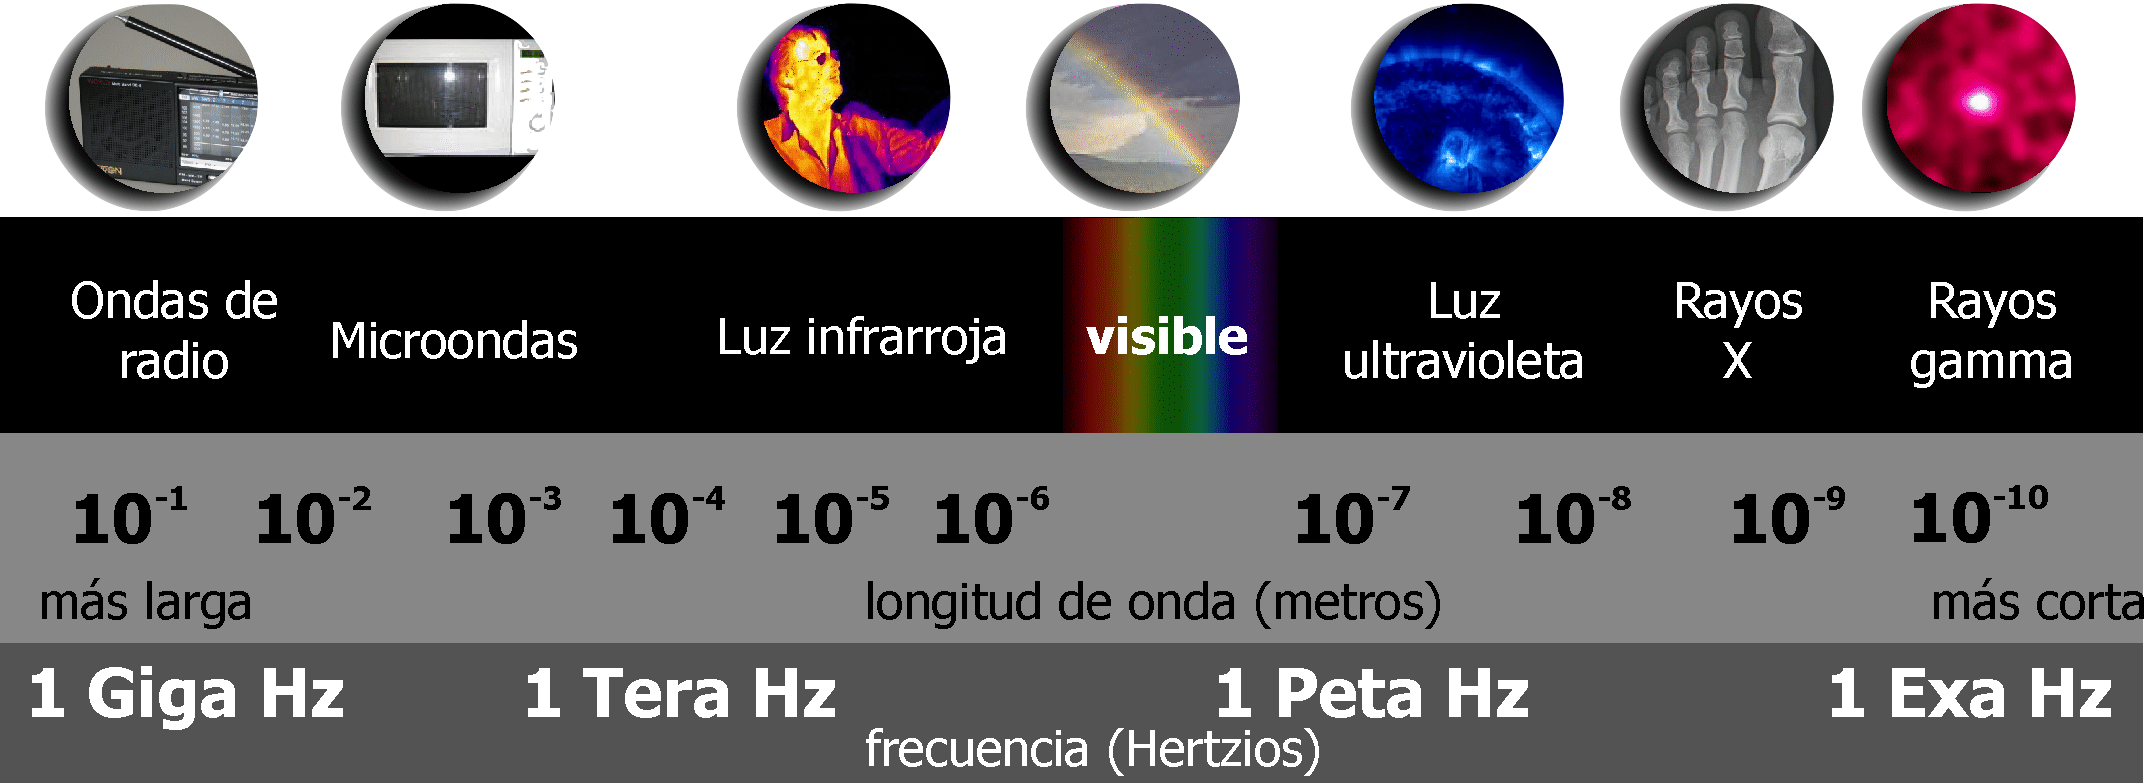
\includegraphics[width=1\textwidth]{imagenes/imagenes22/T22IM01.png}
	\end{figure}

El electromagnetismo abarca diversos fenómenos del mundo real como por ejemplo la luz. La luz es un campo electromagnético oscilante que se irradia desde partículas cargadas aceleradas. Aparte de la gravedad, la mayoría de las fuerzas en la experiencia cotidiana son consecuencia de electromagnetismo.
\end{myalertblock}


\chapter{Carga y Campo eléctricos}

\vspace{-4mm} %**********************************************
\section{Esbozo histórico}

\vspace{-4mm} %**********************************************
$\blacktriangleright$ \textbf{Thales} de Mileto (624 a. C., 546 a. C.): 

--- Una barilla de ambar, frotada con un paño, atrae pedacitos de paja $\to$ efecto eléctrico.

--- La magnetita atrae al hierro $\to$ efecto magnético.

$\blacktriangleright$ Chistian  \textbf{Orested} (1820), físico danés: la corriente eléctrica que pasa por un hilo desvía la aguja magnética de una brújula $\to$ relación entre electricidad y magnetismo.

$\blacktriangleright$ James Clerk  \textbf{Maxwel} (1862), físico inglés: edificó y condensó en 4 fórmulas matemáticas las teorías del electromagnetismo. Unificó en una sola teoría la óptica y el electromagnetismo (la luz es una pequeña parte del espectro electromagnético).

$\blacktriangleright$ Heinrich Rudolf  \textbf{Hertz} (1883), físico alemán: demostró experimentalmente que en su laboratorio era capaz de crear ondas maxwelianas o electromagnéticas, confirmando lo que decía Maxwell 20 años antes.

$\blacktriangleright$ Hendrik Antoon  \textbf{Lorentz} (1902), físico holandés: aclaró conceptualmente la teoría de Maxwell


\section{Carga eléctrica}

Los antiguos griegos sabían ya, hacia el año 600 A de C, que el ámbar, frotado con lana, adquiría la propiedad de atraer cuerpos ligeros (hierba seca, papel, etc.). Al interpretar hoy esta propiedad se dice que el ámbar está electrizado, o que posee carga eléctrica, o que está cargado eléctricamente. Estos términos se derivan del griego, `elektron' que significa ámbar.

En experiencias se utilizan corrientemente una barra de ebonita en lugar del ámbar y una piel. Si después de frotar la ebonita con la piel la acercamos a una bola de corcho que cuelga de una cuerda. Se observa que la bolita de corcho es atraída hacia la varilla (figura a). El experimento análogo realizado con una barra de vidrio frotada con seda dará el mismo resultado (figura b). Por otra parte, si se tienen dos esferas de corcho que previamente han sido "tocadas" cada una por una barra de ebonita previamente frotada con piel. Ambas se repelen (figura c). Lo mismo ocurre si el mismo experimento es realizado con vidrio (figura d).
Ahora, si una de las bolas de corcho ha estado en contacto con la ebonita electrizada, cuando se coloca cerca de otra que ha mantenido contacto con el vidrio electrizado, se observa que se atraen (figura e).

\begin{figure}[H]
		\centering
		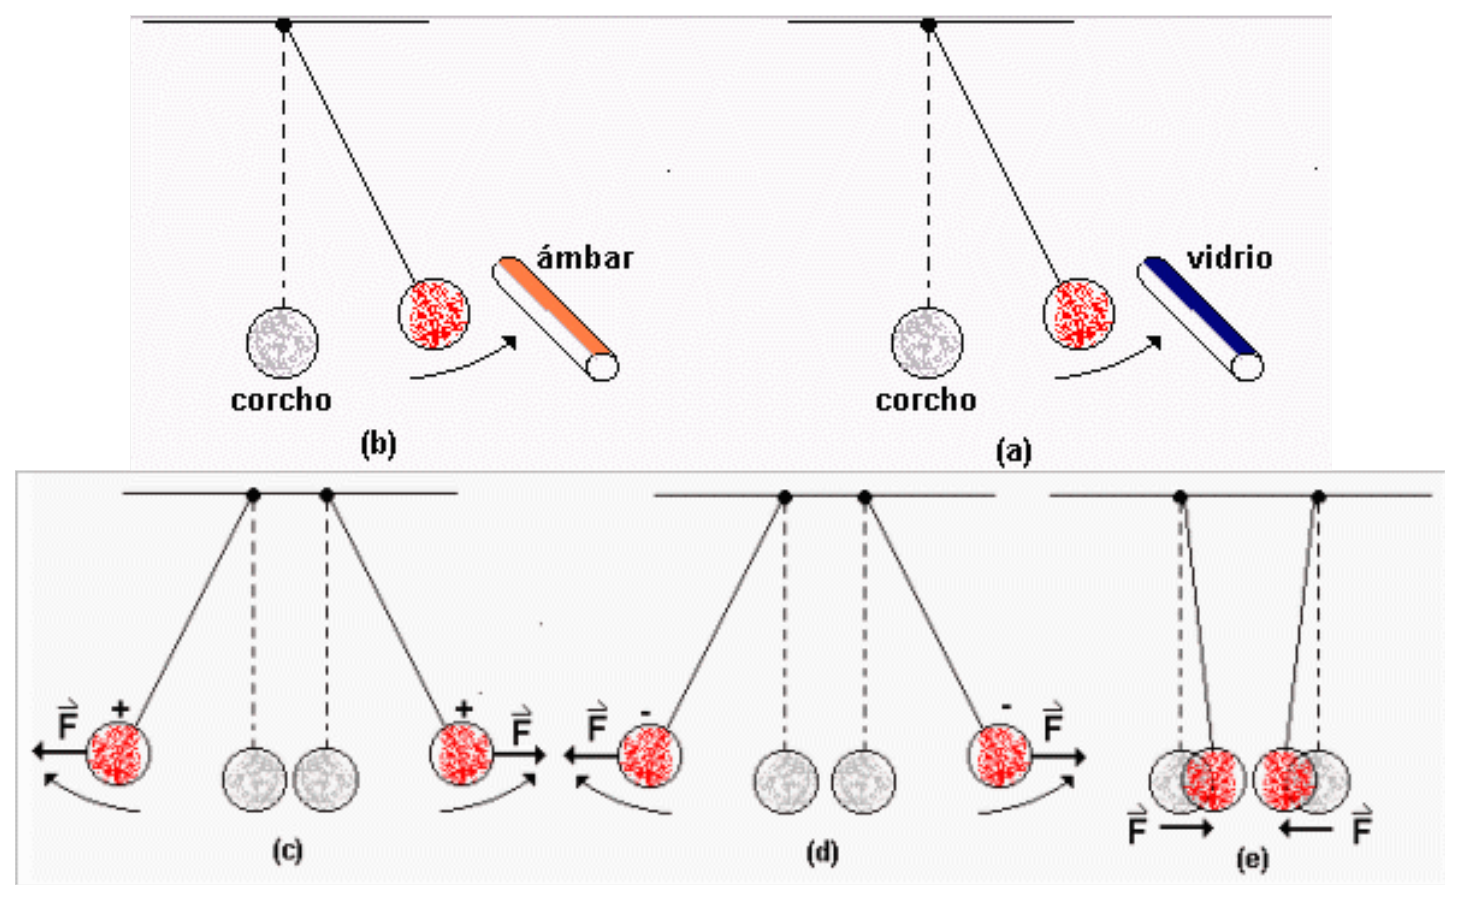
\includegraphics[width=1\textwidth]{imagenes/imagenes22/T22IM02.png}
	\end{figure}

Diremos que las primeras experiencias en las que el ambar o el vidrio atraen al corcho son debidas a una propiedad que se llama \emph{electrización}.

Esto lleva a la conclusión de que hay dos clases de electrización o cargas eléctricas, a las cuales Benjamín Franklin (1706-1790) les asignó los nombres de electrización negativa o carga \emph{negativa} la que posee la ebonita frotada con piel y de electrización positiva o carga \emph{positiva} la que posee el vidrio después de frotado con seda.

Como conclusión de los eventos con bolas de corcho se llega a dos resultados fundamentales: 1) cargas de igual signo se repelen; 2) cargas de distinto signo se atraen.

Tales interacciones atractivas o repulsivas de origen eléctrico coexisten con la interacción gravitatoria de atracción y, Experimentalmente se comprueba que la interacción eléctrica es \emph{mayor} que la de la interacción gravitaroria.

Si acercamos ambas varitas frotadas, vidrio y ambar, a la pelotita de corcho, apenas se siente atracción, los efectos se contrarrestan. Teóricamente, todos los cuerpos materiales deben estar constituidos de forma tal que tengan la misma electricidad negativa que positiva, es decir, que sean \emph{neutros}.

\begin{miparrafodestacado}
	\textbf{\emph{La interacción gravitaroria siempre es atractiva, en cambio, la interacción eléctrica puede ser atractiva o repulsiva}}.
\end{miparrafodestacado}

\begin{figure}[H]
		\centering
		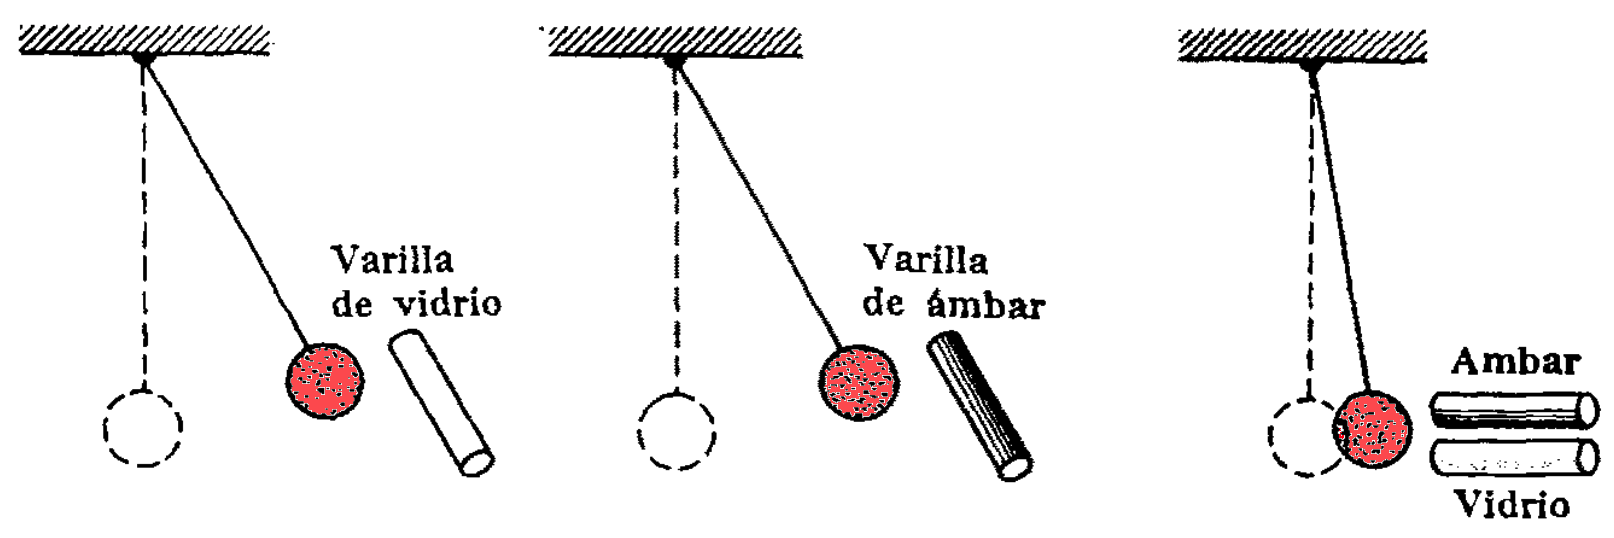
\includegraphics[width=1\textwidth]{imagenes/imagenes22/T22IM03.png}
	\end{figure}

Si acercamos la barra de ambar a dos péndulos con lentejas de corchos y, luego, acercamos estos péndulos observamos que las bolitas de corcho se repelen. Lo mimo ocurre si lo hacemos con la varita de vidrio, pero si acercamos cada péndulo a cada una de estas varitas, al acercar ahora los péndulos observamos que se atraen.

\begin{figure}[H]
		\centering
		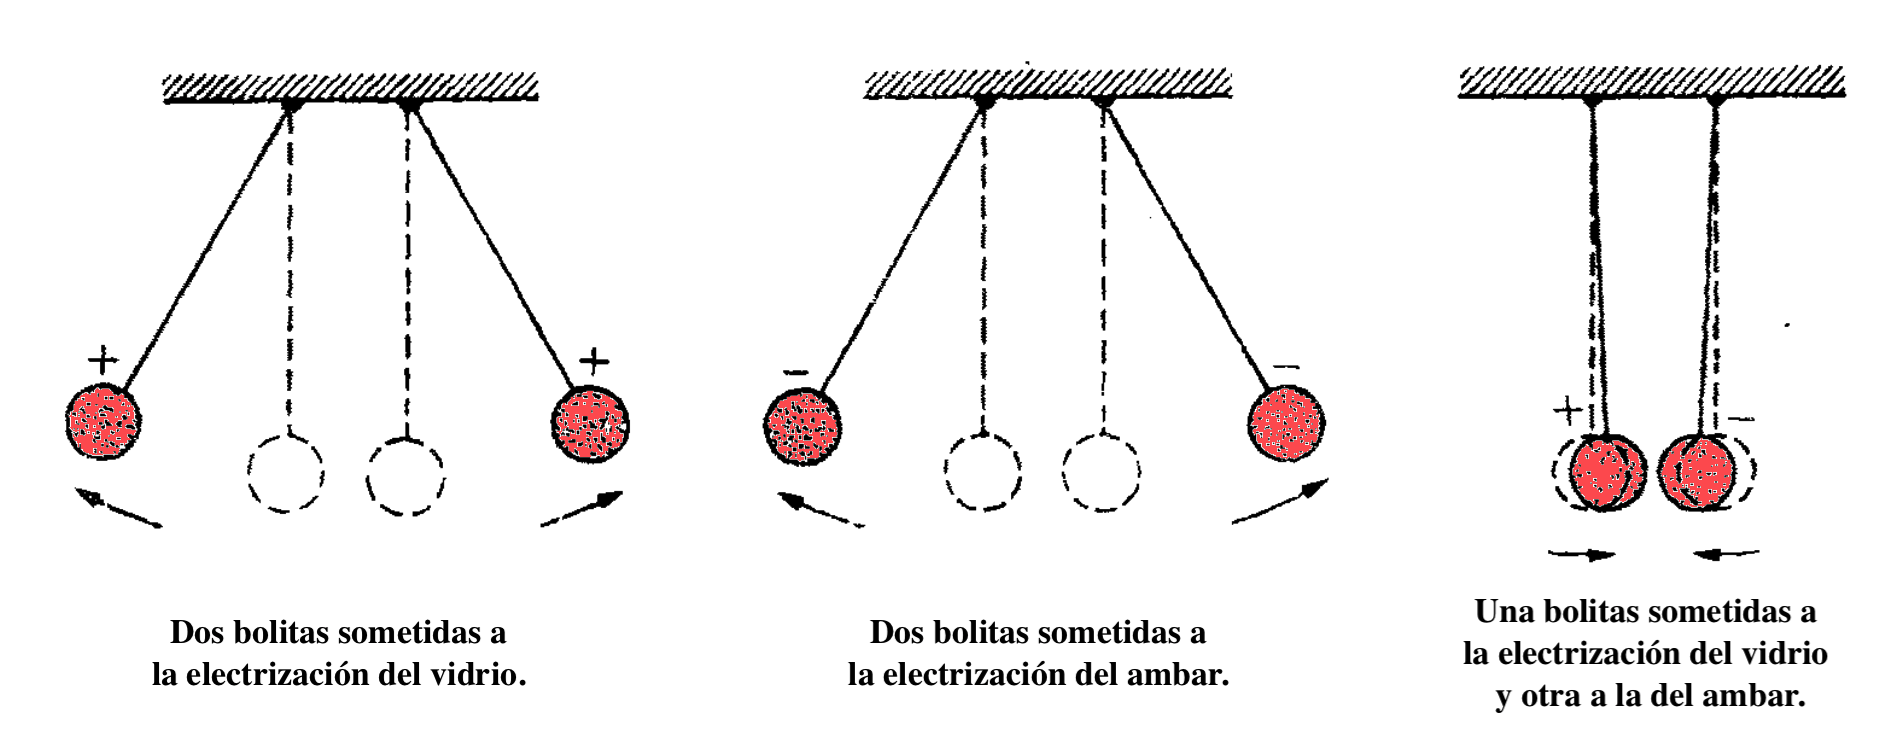
\includegraphics[width=1\textwidth]{imagenes/imagenes22/T22IM04.png}
	\end{figure}

\begin{miparrafodestacado}
Experimentalmente se comprueba que \textbf{\emph{los cuerpos electrizados con el mismo signo se repelen y con distinto signo se atraen.}}
\end{miparrafodestacado}

Del mismo modo que en gravitación introducimos como magnitud activa \emph{la masa}, ahora, para la interacción eléctrica diremos que la magnitud activa el \emph{la carga} eléctrica. A diferencia de la masa, \emph{la carga puede ser positiva o negativa}.

Diremos que un cuerpo está electrizado positivamente porque se le han cedido cargas negativas, análogamente para cuerpos electrizados positivamente. 

Vamos a definir operacionalmente el concepto de \emph{carga eléctrica}:

\begin{multicols}{2}
$d$ es lo suficientemente grande comparado con las dimensiones de los cuerpos cargados $Q, \ q,\ \textcolor{gris}{(q')}$ como para que podamos considerarlos  como puntuales.

\begin{figure}[H]
		\centering
		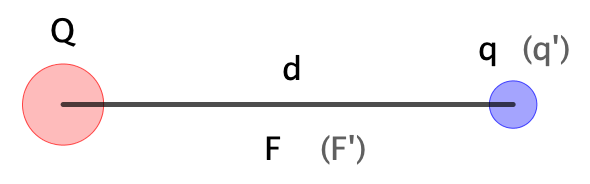
\includegraphics[width=.5\textwidth]{imagenes/imagenes22/T22IM05.png}
	\end{figure}	
\end{multicols}
Con los cuerpos $Q \text{ y } q$ determinamos la fuerza $F$. Intercambiamos los cuerpos $q \text{ y } q'$ y medimos la fuerza $F'$. Por definición diremos que ls cuerpos  $q \text{ y } q'$ tienen unas cargas tal que verifican la relación $\ \dfrac F {F'}=\dfrac q {q'}$. Atribuimos a $q'$ la carga unidad y así podemos calcular cantidades relativas de carga.

La carga eléctrica es un \emph{observable} que no se puede poner en función de ningún otro por lo que es una \emph{magnitud fundamental}. Los cuerpos están definidos por su masa y su carga.

En la naturaleza se observa un hecho experimental que siempre se cumple:

\begin{miparrafodestacado}
\textsf{Principio natural de conservación de la carga:}	\textbf{\emph{``En todo sistema físico aislado la carga se conserva''}}.
\end{miparrafodestacado}

\section{Conductores y aislantes}

Tomamos un metal, por ejemplo el $Cu$, se le frota con una piel y se acerca a un péndulo con lenteja de corcho: observamos que el corcho no sufre ninguna atracción por lo que concluimos que la naturaleza del $Cu$ es distinta a la del ambar o a la del vidrio.

Podría ocurrir que, o bien el cobre no almacena electricidad, o bien se le escapa. Experimentalmente se comprueba que la segunda hipótesis es válida, pues si se aísla la varilla de cobre con un mango de madera sí que atrae.

Habrán, pues, dos familias de materiales, una que al ser frotados se cargan y no desaparece por el cuerpo y otra, que llamaremos \emph{metálicos}, que al frotarlos y cogerlos con la mano, la carga desaparece por el cuerpo humano y va a la tierra. A la primera familia se les llama \textbf{\emph{ dieléctricos o aislantes}} y a la segunda \textbf{\emph{conductores}}.

Solo en los cuerpos metálicos la carga es capaz de circular por ellos: \emph{efecto Hall}. A esa carga \emph{negativa} que se mueve le llamaremos \textbf{\emph{electrón}}. En cuerpos no metálicos, \emph{electrolitos}, también se puede mover la carga positiva.

En la naturaleza no existe ningún cuerpo que sea totalmente aislante. Hay una tercera familia, los cuerpos \textbf{\emph{semiconductores}} que no son tan aislantes como los \emph{dieléctricos} ni tan poco como los \emph{conductores}. ($Si,\ Ge$). Los cuerpos \emph{semiconductores} los estudia la \emph{física cuántica}.

\section{Ley de Coulomb}

Toda la \emph{electrostática\footnote{La electrostática es el estudio de la electricidad que no cambia con el tiempo.}} surge de la \emph{ley de Coulomb} (1785), es una ley experimental.

Coulomb, ensayando con cuerpos cargados, llegó a las siguientes conclusiones:
\begin{itemize}
\item La interacción eléctrica que se ejerce entre dos cuerpos de dimensiones pequeñas comparada con la distancia que los separa es:
	\begin{enumerate}[a) ]
	\item Directamente proporcional a cada una de las cargas.
	\item Inversamente proporcional al cuadrado de la distancia que las separa.
	\item La interacción se dirige a lo largo de la línea que una ambas cargas.
	\item Dicha interacción es atractiva para cargas de signos contrarios y repulsiva para cargas del mismo	 signo.
	\end{enumerate}
\item Cuando se tienen más de dos cargas, la interacción que el resto de cargas produce sobre una de ellas cumple el principio de superposición o la ley del paralelogramo (suma vectorial).

\begin{miparrafodestacado}
	\textbf{Principio de superposición}: \emph{Si en una región del espacio existe más de un cuerpo cargado, al colocar en dicha región una nueva carga de prueba $q$ , la intensidad de la fuerza electrostática a la que esta carga se verá sometida será igual a la suma de la intensidad de las fuerzas que ejercerían de forma independiente sobre ella cada una de las cargas existentes.}
\end{miparrafodestacado}

\end{itemize}

\begin{equation}
\label{ley-Colulomb}	
\subrayado{ \ \boxed{\ \boldsymbol{\overrightarrow{F}\ = \ K_e\ \dfrac {q_1 \ q_2}{r^2}\ \vec u_r }  \ } \ } \qquad \text{Ley de Coulomb}
\end{equation}

donde $k_e=10^{-7}c^2 \approx 9\times 10^9\ UI \ $\footnote{$c$ es la velocidad de la luz en el vacío y $UI$ son unidades internacionales.}

Ya estamos en condiciones de definir la unidad de carga:

La unidad internacional de carga es el \emph{\textbf{Coulomb}}, $C$, que se define del siguiente modo:

\begin{miparrafodestacado}
Se dice que dos cuerpos idénticos tienen la carga de un coulomb, $1 \ \mathrm{C}$, cuando colocados a una distancia de $1\ \mathrm{m}$ aparece sobre ellos una fuerza de repulsión de $8.9874\times 10^9\ \mathrm{N}$.	
\end{miparrafodestacado}

Con esto, $\ K_e=10^{-7} c^2=8.9874\times 10^9\ UI=8.9874\times 10^9 \ \mathrm{N\ C}^{-2}\mathrm{m}^2$

Es conveniente definir la constante eléctrica de otro modo: $\boldsymbol{\ k_e=\dfrac 1 {4\pi \varepsilon_0}}$

donde $\ \varepsilon_0\ $ es una \emph{constante universal} llamada \emph{permitividad del vacío} o constante dieléctrica del vacío y en el $SI$ tiene un valor de $\ \varepsilon_0=8.854\times 10^{-12}\ \mathrm{N\ m}^{2}\mathrm{C}^{-2}$, por lo que la ley de Coulomb en el $SI$ se puede escribir como:

\begin{equation}
\label{ley-Colulomb-SI}	
\subrayado{ \ \boxed{\ \boldsymbol{\overrightarrow{F}\ = \dfrac {q_1 \ q_2}{4\pi \ \varepsilon_0\ r^2}\ \vec u_r }  \ } \ } \qquad \text{Ley de Coulomb en el }SI
\end{equation}

\section{Campo y potencial eléctricos}

\textbf{Campo electrostático}: Depositamos una carga eléctrica, \emph{en reposo}, en una región determinada del espacio. Si sobre esa carga actúa una fuerza eléctrica decimos que en esa región existe un \emph{campo eléctrico}.

La fuerza $\vec F$ que aparece es directamente proporcional a la \emph{carga prueba} $q$ (carga que depositamos en el espacio). La constante de proporcionalidad es la \emph{intensidad del campo eléctrico} en el punto del espacio que ocupa la carga prueba.

\begin{equation}
\label{def-campo-electrico}
\boldsymbol{ \vec F \ = \ q\ \vec E}	
\end{equation}

En el caso particular de que solo haya una carga $q_1$ que altera el medio, crea el campo, de acuerdo con la ley de Coulomb, tenemos:

$\vec F=\dfrac{qq_1}{4\pi \varepsilon_0 r^2} \ \vec u_r= q \ \vec E$, tendremos que

\begin{equation}
\label{campo-electrico-carga-puntual}
\subrayado{ \ \boldsymbol{ \vec E \ = \ \dfrac{q_1}{4\pi \varepsilon_0 r^2} \ \vec u_r } \ } \qquad \text{ \footnotesize{Campo eléctrico  creado por una carga puntual}\normalsize{.}}	
\end{equation}

Puesto que Coulomb observó que en la interacción eléctrica se cumplía el principio de superposición, ley del sacacorchos, tendremos que \emph{el campo eléctrico creado por una distribución finita de $N$ cargas} será:

$$\vec E = \dfrac{q_1}{4\pi \varepsilon_0 r_1^2} \ \vec u_{r_1} +
\dfrac{q_2}{4\pi \varepsilon_0 r_2^2} \ \vec u_{r_2} + \cdots +
\dfrac{q_N}{4\pi \varepsilon_0 r_N^2} \ \vec u_{r_N} =
\displaystyle \dfrac{1}{4\pi \varepsilon_0} \sum_{i=1}^N \dfrac{q_i \vec u_{r_i}}{r_i^2} $$
 

Para una distribución continua de cargas, que es lo que normalmente ocurre en la naturaleza en problemas macroscópicos, tendremos:

\begin{multicols}{2}
$P$ es el punto donde colocamos la carga prueba para calcular el campo que crea la distribución de cargas $Q$.

$\dd \vec E=\dfrac{\dd q}{4\pi \varepsilon_0 r^2}\vec u_r$, luego
\begin{figure}[H]
		\centering
		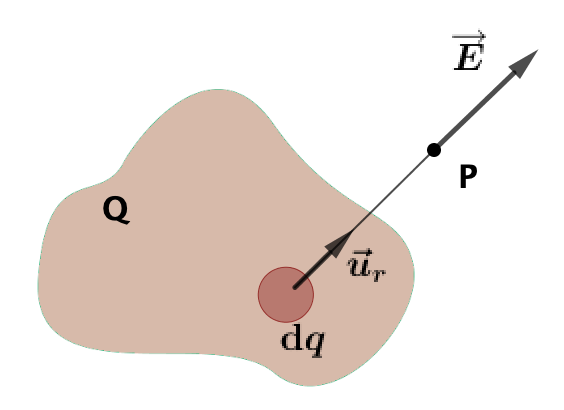
\includegraphics[width=.45\textwidth]{imagenes/imagenes22/T22IM06.png}
	\end{figure}	
\end{multicols}

\begin{equation}
 \boldsymbol{\vec E\ = \ \dfrac{1}{4\pi \varepsilon_0} \int_Q \dfrac{\dd q \ \vec u_r}{r^2}}
\end{equation}

Densidad eléctrica de carga: $\dd q= \rho \dd \tau \quad \to 
\quad \displaystyle \vec E =  \dfrac{1}{4\pi \varepsilon_0} \int_\tau \dfrac{\rho \ \dd \tau \ \vec u_r}{r^2}$

En el caso particular de que $\rho=cte \quad \to \quad \displaystyle \vec E =  \dfrac{\rho}{4\pi \varepsilon_0} \int_\tau \dfrac{ \dd \tau \ \vec u_r}{r^2}$

\emph{Significado físico:} \textbf{el campo eléctrico es central}, luego es \textbf{conservativo}, como la fuerza eléctrica. Todo lo que vimos que cumplían los campos conservativos será válido para el campo eléctrico.

$\overrightarrow{F}$ conservativa $\to \displaystyle \oint \vec F \cdot \dd \vec l =0=\oint \vec E \cdot \dd \vec l$, pues $q$ es $cte$. Del mismo modo, $\overrightarrow{E}$ conservativo $ \to \overrightarrow{\grad} \times \overrightarrow{E} = \vec 0 \to  \subrayado{\boldsymbol {\overrightarrow{E}=-\overrightarrow{\grad} V}}$, donde $V$ es el \textbf{potencial eléctrico}, $\boldsymbol{V=\dfrac{\mathcal E_p}{q} \leftrightarrow \mathcal E_p =qV}$. En el $SI$, $V$ se expresa en Joules/Coulomb$=J/C=V$, que recibe el nombre de \textbf{volt}\footnote{el nombre de \emph{volt} es en honor a Alessandro Volta, quien en 1800 inventó la pila voltaica, la primera batería química.}

\emph{En los campos conservativos, las líneas de campo son siempre perpendiculares a las superficies equipotenciales en cada punto.}

\vspace{5mm} %******************************
\large{\textbf{Casos particulares}}

\subsection{Potencial asociado al campo eléctrico creado por una sola carga}


\begin{multicols}{2}
\normalsize{Potencial} $V_1$ que la carga $q_1$ crea en el punto $P$, a distancia $\vec r_1$ del lugar que ocupa la carga: 

$\displaystyle \vec E_1=\dfrac{q_1}{4\pi \varepsilon_0 r^2}\vec u_r=-\dv{V_1}{r}\vec u_{r_1}$

$\displaystyle \dv{V_1}{r}=-\dfrac{q_1}{4	\pi \varepsilon_0 r^2}$
\begin{figure}[H]
		\centering
		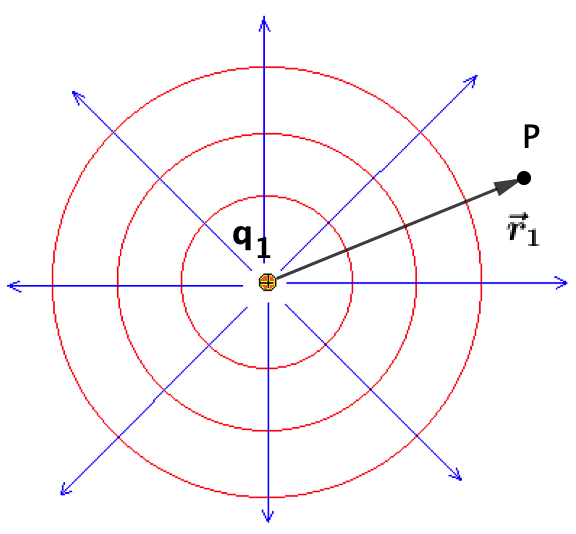
\includegraphics[width=.4\textwidth]{imagenes/imagenes22/T22IM07.png}
	\end{figure}	
\end{multicols}

\normalsize{$V_1=\displaystyle \int \dfrac{q \ \dd r}{4	\pi \varepsilon_0 r^2}=\dfrac{q_1}{4	\pi \varepsilon_0 r} + \mathcal C$, siendo $\mathcal C$ la constante de integración, arbitraria como ocurría con la energía potencial.}

Elegimos la constante arbitrario de modo que el potencial que crea una carga puntual en el infinito sea cero: $V_1(\infty)=0=\mathcal C$, de este modo:

\begin{equation}
\boldsymbol{V_1 \ = \ \dfrac{q_1}{4	\pi \varepsilon_0 r}}	
\end{equation}

\subsection{Potencial creado por una distribución discreta de cargas}

\begin{multicols}{2}

$\quad$

Generalizando la expresión anterior:


\begin{figure}[H]
		\centering
		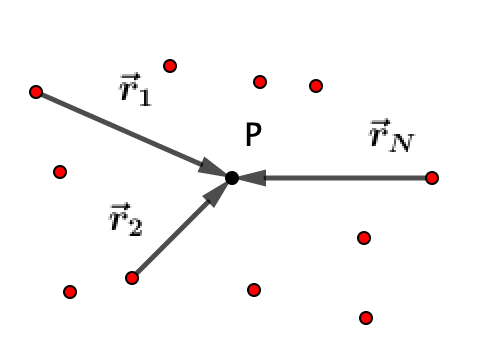
\includegraphics[width=.3\textwidth]{imagenes/imagenes22/T22IM08.png}
	\end{figure}	
\end{multicols}

\begin{equation}
\boldsymbol{ V=}\sum_{i=1}^N V_i = \boldsymbol{ \dfrac {1}{4\pi \varepsilon_0} \sum_{i=1}^N \dfrac {q_i}{r_i} }
\end{equation}

\subsection{Potencial creado por una distribución continua de cargas}

\begin{multicols}{2}
\begin{eqnarray}
\boldsymbol{V\ =}\ \dfrac {1}{4\pi \varepsilon_0}\int_Q \dfrac{dd q}{r}   \nonumber \\
\boldsymbol{=\ \dfrac {1}{4\pi \varepsilon_0} \int_\tau \dfrac{\rho \ \dd \tau}{r}} 	
\end{eqnarray}
\begin{figure}[H]
		\centering
		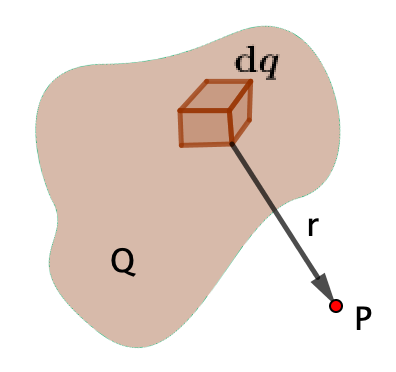
\includegraphics[width=.25\textwidth]{imagenes/imagenes22/T22IM09.png}
	\end{figure}	
\end{multicols}


\begin{equation}
\text{si } \rho=cte \ \to \ 	\boldsymbol{V=\ \dfrac {\rho}{4\pi \varepsilon_0} \int_\tau \dfrac{ \dd \tau}{r}}
\end{equation}

\subsection{$V$ en una región en que $\vec{E}$ es constante}
\label{EV-Ecte}

$\displaystyle \overrightarrow{E}=\vec i\ E= \overrightarrow{cte} = -\vec i\ dv{V}{x} \to \dd V=-E \dd x \to V=-Ex+\mathcal C$

\normalsize{Elegimos la constante de modo que $V(0)=0=\mathcal C$, por lo que:}

\begin{equation}
\boldsymbol{V \ = \ - E\ x}	
\end{equation}

\vspace{-5mm} %*****************************************
\begin{figure}[H]
	\centering
	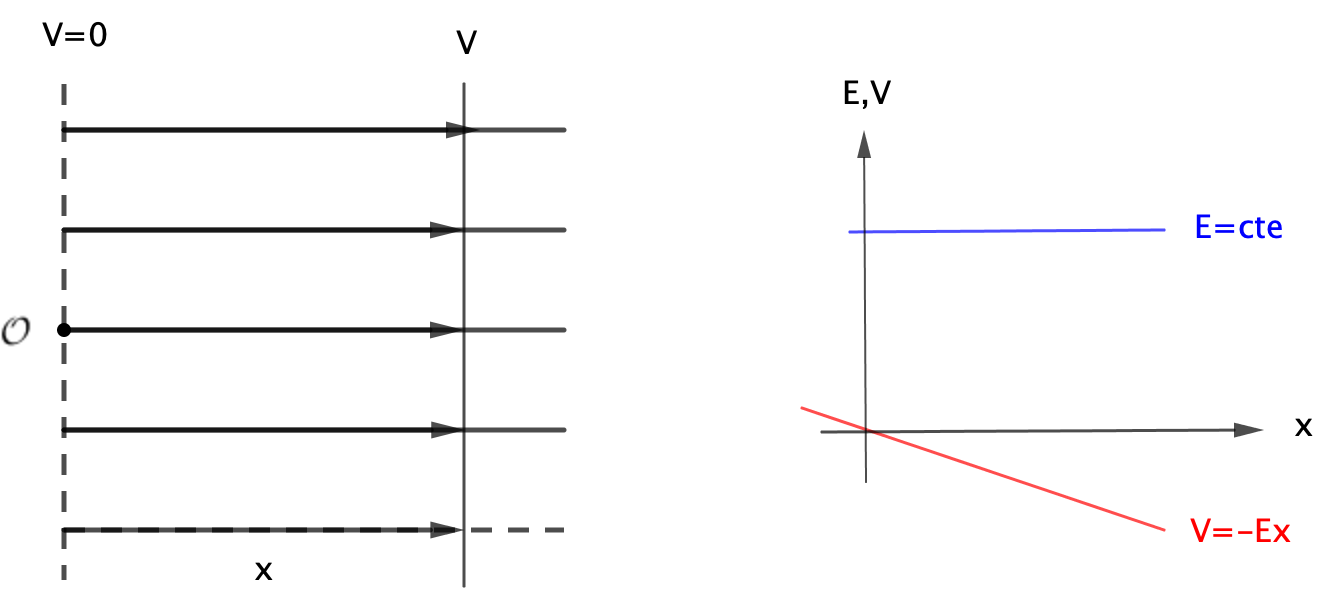
\includegraphics[width=.9\textwidth]{imagenes/imagenes22/T22IM10.png}
\end{figure}
\vspace{-5mm} %*****************************************
Esto ocurre, por ejemplo, con las placas de un condensador plano paralelo.

Observación, otras unidades para el campo eléctrico: de esta ecuación observamos que $E=-\dfrac V x$ luego las unidades de $E$ serán $ \dfrac {\mathrm{V}} {\mathrm{m}}=\dfrac{\mathrm{N}}{\mathrm{C}}$, obtenidas a partir de la definición de campo eléctrico $F=qE$. Usualmente su utliza más $ \mathrm{N\ m}^{-1}$ que  $\mathrm{N\ C}^{-1}$, pero son la misma unidad.

\section[Cuantización de la carga. Experimento de Millikan]{Cuantización de la carga. Experimento de Millikan\sectionmark{experimento de Millikan}}
\sectionmark{experimento de Millikan}

Podemos encontrar la unidad de carga de modo que no haya ninguna menor que ella con procedimientos macroscópicos.


Robert Andrews Millikan (1909), físico estadounidense, descubrió que había una \emph{unidad última de carga}: `experimento de la gota de aceite de Millikan'.

\begin{figure}[H]
	\centering
	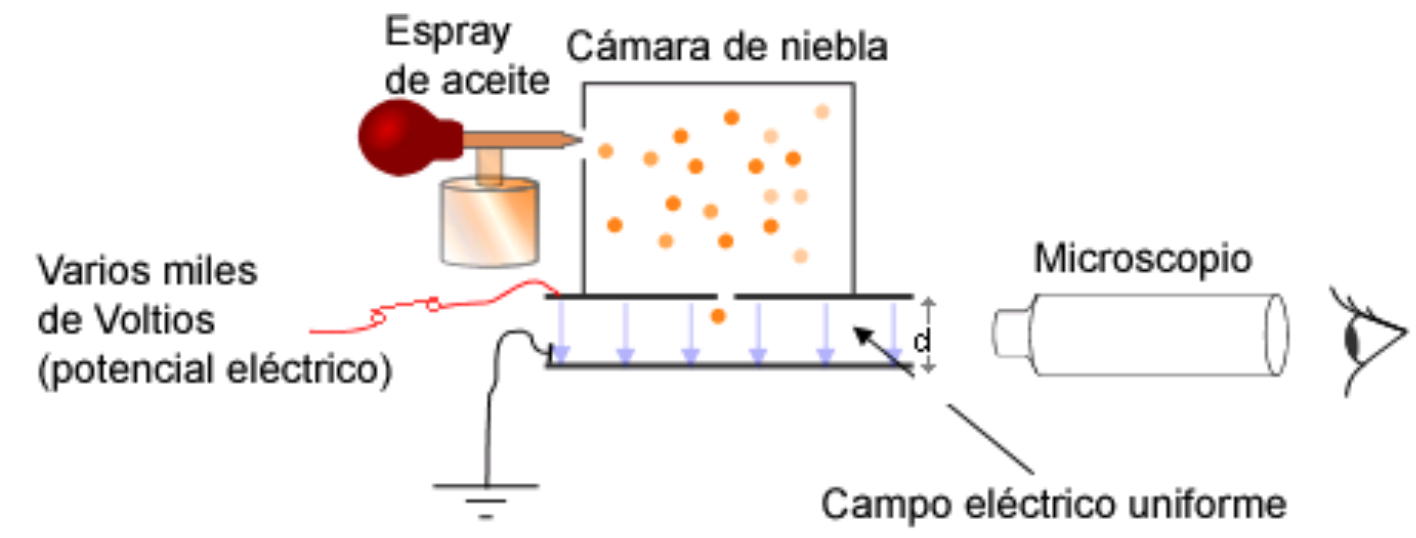
\includegraphics[width=.9\textwidth]{imagenes/imagenes22/T22IM11.png}
\end{figure}

Cuando aún no se ha conectado la bateria que proporciona el potencial de miles de voltios no hay campo eléctrico y las fuerzas que actúan, eligiendo como sentido positivo el que va hacia abajo:

$mg-\rho_0 \tau g -6\pi r \eta v= ma$, donde el primer término aparece el peso, después el empuje de Arquímedes y, en tercer lugar, la fuerza de Stokes de rozamiento (contraria al movimiento), todas ellas son la fuerza resultante que por Newton son masa por aceleración \textcolor{gris}{($v$ es la velocidad con que cae la gota, $m=\rho g$)}.

Considerando $\ \rho>>\rho_0 \to \tau g (\rho-\rho_0)\approx \tau g \rho$. En el momento que se alcanza la velocidad límite, $v=v_L=cte \to a=0$ y tendremos:

$\tau \rho g-6\pi r \eta v_L=0$, $\ v_L \ (*)$ la podemos determinar experimentalmente.

Conectamos, ahora, el campo eléctrico y aparece la fuerza eléctrica: $\tau \rho g \pm q E -6\pi r \eta v$.

Como las gotas de aceite se cargan positivamente, tendremos $\tau \rho g + q E -6\pi r \eta v=ma$

Se alcance una nueva velocidad límite $v'_L \to a =0 \Rightarrow $

$\tau \rho g + q E -6\pi r \eta v'_L=0 \ \to \ q=\dfrac{6\pi r \eta v'_L-\tau \rho g}{E}$

D lo obtenido antes de conectar el campo $\ (*) \ \to \ \tau \rho g=6\pi r \eta v_L$, tendremos

\begin{equation}
q\ =\ \dfrac{6\pi r \eta (v'_L-v_L)}{E}	
\end{equation}

y podemos determinar la carga $q$ asociada al aceite.

Conclusión: la carga $q$ asociada a la gota de Millikan siempre toma el mismo valor que es múltiplo o igual a:

\begin{equation}
\boldsymbol{e \ = \ 1.0621\times 10^{-19} \ \mathrm{C}};	 \qquad \textbf{carga elemental}
\end{equation}

\textcolor{gris}{Se suele observar que esta gota, en vez de caer de modo continuo experimenta subidas y bajadas. Ello es debido a su interacción con los rayos cósmicos.}

\begin{figure}[H]
	\centering
	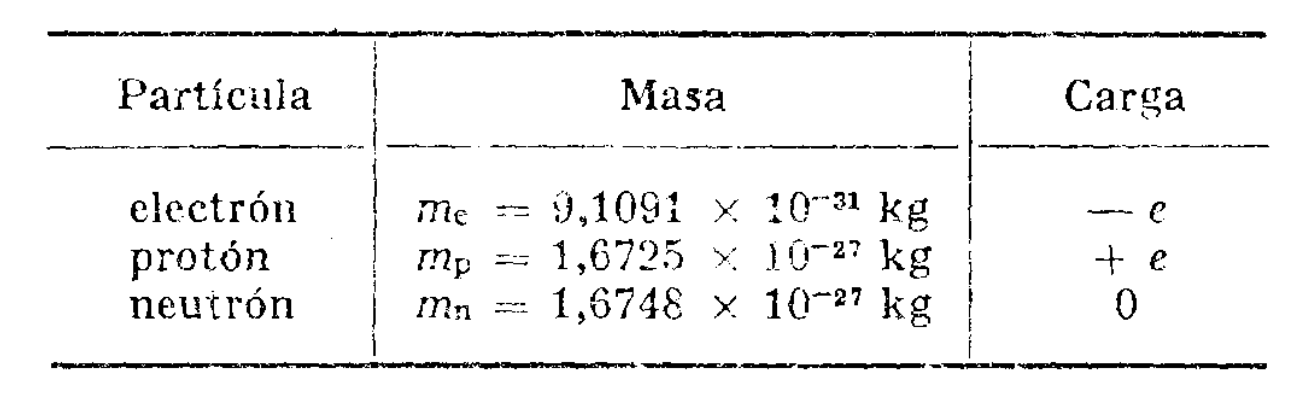
\includegraphics[width=1\textwidth]{imagenes/imagenes22/T22IM14.png}
\end{figure}


\begin{figure}[H]
	\centering
	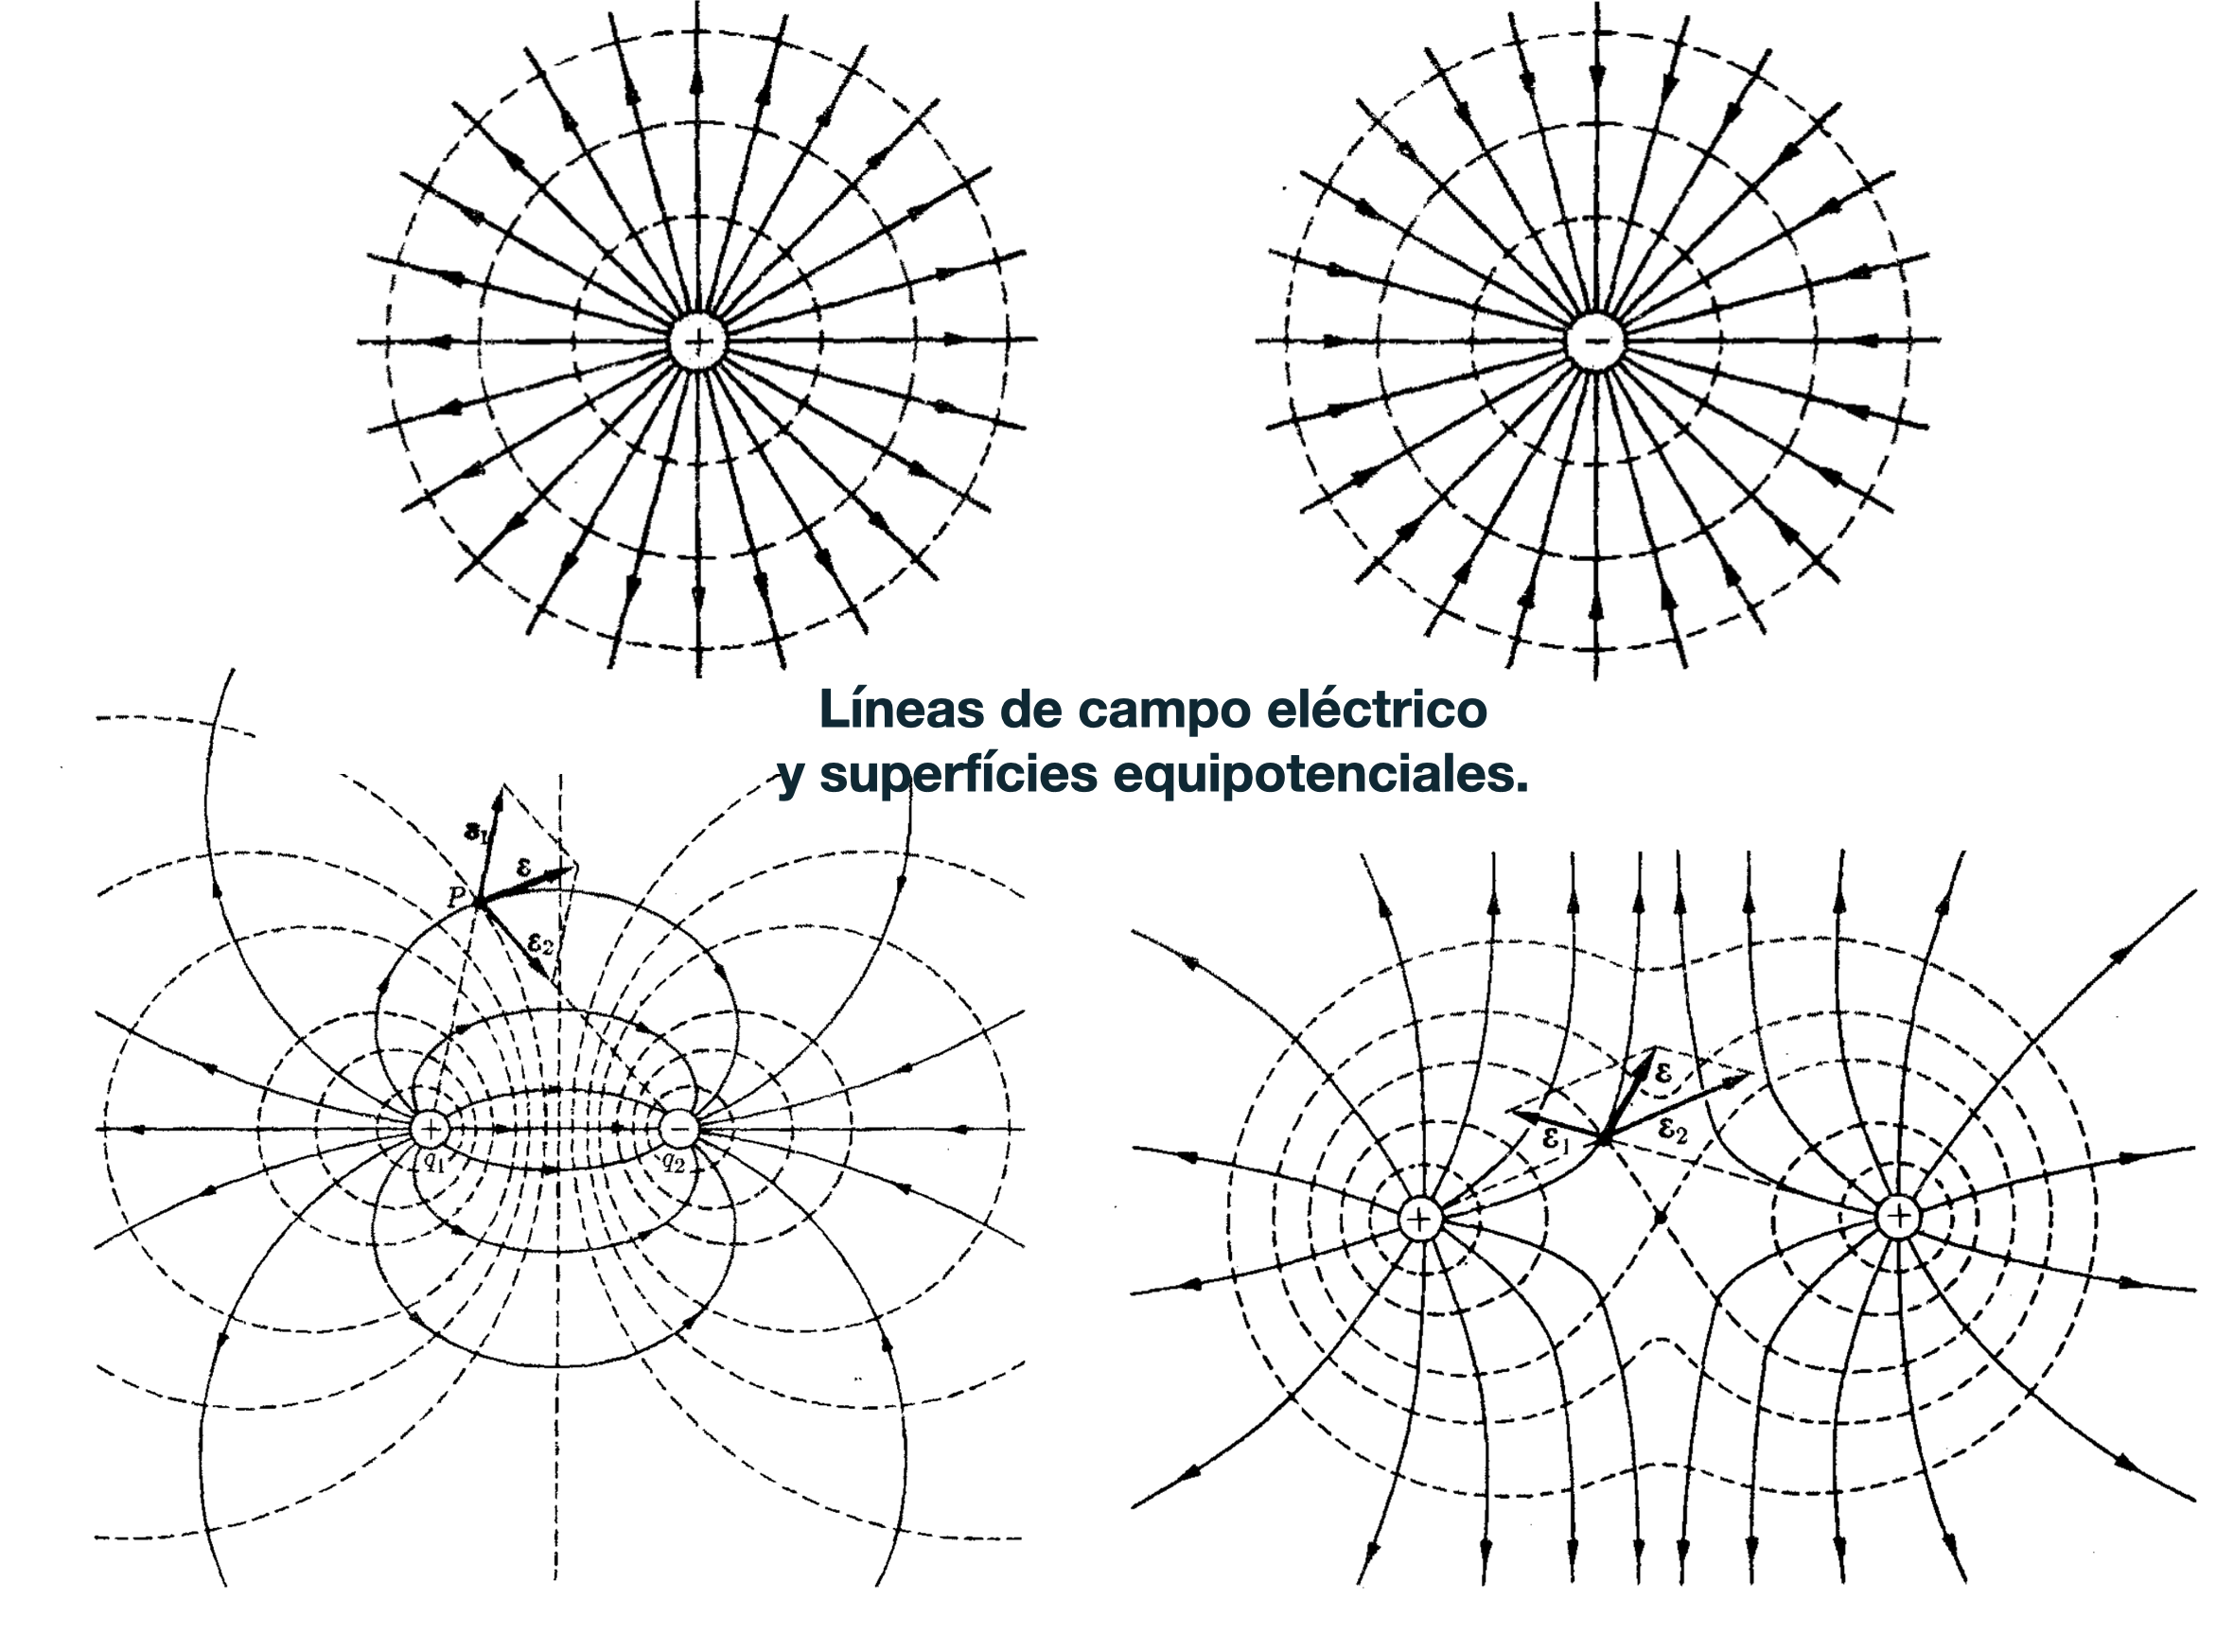
\includegraphics[width=1\textwidth]{imagenes/imagenes22/T22IM13.png}
\end{figure}

\section{Problemas}
\begin{prob}
	\normalsize{Una partícula $\alpha$ es un núcleo de $He$. Tiene una masa $m=6.64\times 10^{-27}\ \mathrm{Kg}$ y una carga $q=2e^-=3.2\times 10^{-19}\ \mathrm{C}$. Compare la fuerza de repulsión eléctrica entre dos partículas $\alpha$ con la atracción gravitatoria que hay entre ellas.}
	
	Dato: $G=6.67\times 10^{-11}\ \mathrm{N\ m}^2 \mathrm{kg}^{-2};\ \varepsilon_0=8.854\times 10^{-12} \ \mathrm{N\ m}^2 \mathrm{C}^{-2}$.
\end{prob}
\begin{multicols}{2}
$F_e=\dfrac {q^2} {4\pi \varepsilon_0 r^2};\ $
$F_g=G\dfrac{m^2}{r^2}$

$ \dfrac {F_e} {F_g}=\dfrac {1}{4\pi \varepsilon_0 G} \ \dfrac {q^2}{m^2}= 3.1\times 10^{35}$
\begin{figure}[H]
	\centering
	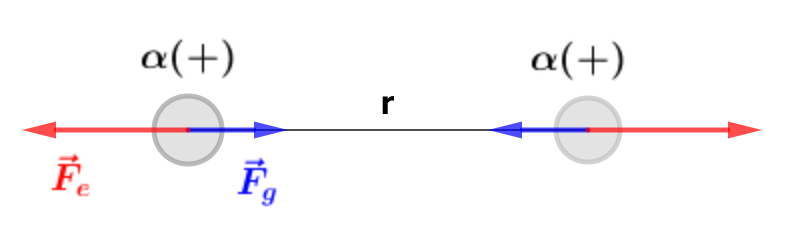
\includegraphics[width=.5\textwidth]{imagenes/imagenes22/T22IM15.png}
\end{figure}	
\end{multicols}

Como se puede observar en esta situación, $F_e \sim 10^{35} F_g$, la fuerza gravitatoria es despreciable por completo en comparación con la fuerza eléctrica. Esto siempre se cumple para interacciones de partículas atómicas y subatómicas y el resultado es independiente de la distancia de separación $r$ de las partículas. Para objetos del mayor tamaño (un ser humano o un planeta), las cargas positiva y negativa son de magnitud casi igual por lo que la fuerza eléctrica neta por lo general es muchísimo menor que la gravitatoria.

\begin{prob}
Entre dos placas planas y paralelas cargadas con cargas iguales y de signos opuestos existe un campo eléctrico uniforme. Se libera un electrón de la superficie de la placa negativa y choca contra la superficie de la placa opuesta, distante $2.0\ \mathrm{cm}$	de la primera, al cabo de $1.5\times 10^{-8}\ \mathrm{s}$. Calcula el campo eléctrico y la velocidad con que el electrón choca contra la superficie de la placa positiva.
\end{prob}

\begin{multicols}{2}
$F=eE=cte=ma$ 

$a=cte:\ MRUA$

$E=\dfrac{ma}{e}$

$MRUA:\ d=\dfrac 1 2 a t^2 \to E=\dfrac me \dfrac {2d}{t^2}$
\begin{figure}[H]
	\centering
	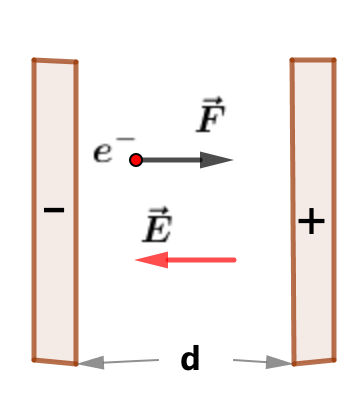
\includegraphics[width=.25\textwidth]{imagenes/imagenes22/T22IM16.png}
\end{figure}		
\end{multicols}

Datos: $\quad m=m_e=9.108\times 10^{-31} \mathrm{kg};\qquad  e=1.602\times 10^{-19}\ \mathrm{C}; \qquad  $

$d=2\times 10^{-2} \ \mathrm{m}; \qquad t=1.5\times 10^{-8}\ \mathrm{s}$

Sustituyendo: $\qquad E\ = \ 0.1012 \ \mathrm{N \ C}^{-1}$

$MRUA: \quad v=at \ \to \ v=\dfrac{2d}{t^2}t=\dfrac{2d}{t}= 1.467\times 10^6 \ \mathrm{m\ s}^{-1}$


\begin{prob}
Cuando una batería se conecta a dos placas conductoras planoparalelas, las cargas resultantes en las placas originan un campo eléctrico entre ellas que es prácticamente uniforme. Las placas están separadas $1.0\ \mathrm{cm}$ y se conectan a una batería de $100\ \mathrm{V}$ creando un campo eléctrico de $1.00\times 10^4\ \mathrm{N\ C}^{-1}$. Suponiendo que $\vec E$ está orientado hacia arriba como muestra la figura adjunta, responde a las siguientes preguntas:

$a)\ $ Si un electrón en reposo se libera el la placa superior, ?`cuál será su aceleración?

$b \ $ ?`Qué rapidez y qué energía cinética adquiere el electrón cuando ha viajado $1.0\ \mathrm{cm}$ hacia la placa inferior?

$c)\ $ ?`Cuánto tiempo tarda en recorrer esa distancia?

Datos: $\quad =m_e=9.108\times 10^{-31} \mathrm{kg};\qquad  e=1.602\times 10^{-19}\ \mathrm{C}; \qquad  $

\begin{figure}[H]
	\centering
	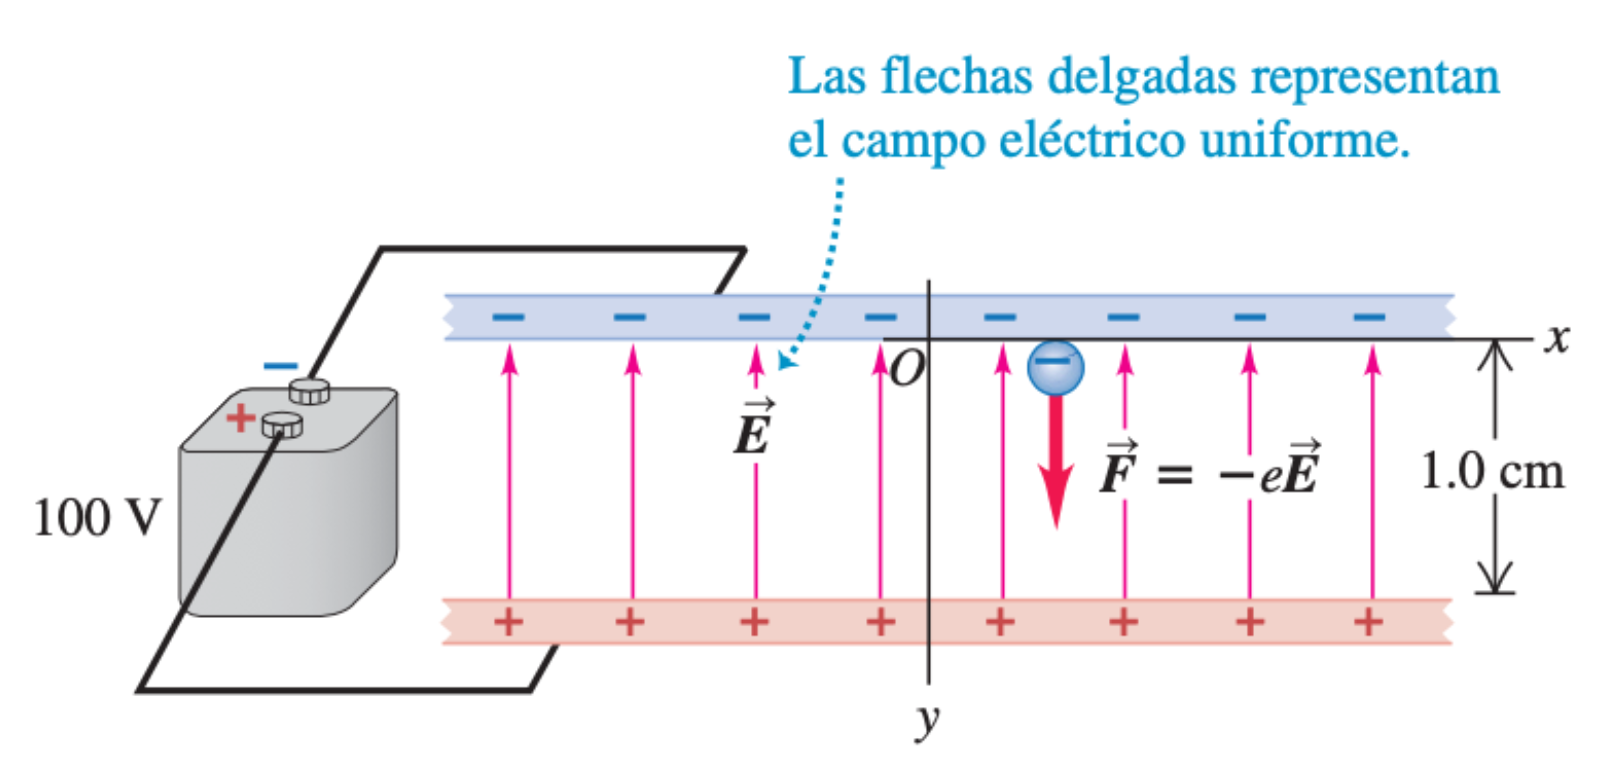
\includegraphics[width=.9\textwidth]{imagenes/imagenes22/T22IM19.png}
\end{figure}
\end{prob}

--- $a)\ $ Movimiento en el eje $y$: $\ \vec E$ hacia arriba; $\vec F$ hacia abajo ya que la carga del electrón es negativa y constante $\to a_y=cte \to MRUA$

$a_y=\dfrac{F_e}{m}=\dfrac{-eE}{m}=\dfrac{-1.6\times 10^{-19} \cdot 1.00\times 10^{4}}{9.11\times 10^{-31}}=-1.76\times 10^{15}\ \mathrm{m\ s}^{-2}$

Obviamente, la fuerza de la gravedad es totalmente despreciable comparada con la fuerza eléctrica.

--- $b)\ $ El electrón parte del reposo por lo que su movimiento solo se produce en el eje $y$ y es un $MRUA$

$v=\sqrt{2a_y y}=\pm \sqrt{2\cdot (-1.76\times 10^{15}) \cdot (-1.0 \times 10^{-2})}=- 5.9\times 10^6 \ \mathrm{m\ s}^{-1}$, en sentido hacia abajo.

$\mathcal E_c=\dfrac 1 2 m v^2=\dfrac 1 2  \cdot 9.11\times 10^{-31} \cdot (-5.9 \times 10^6)^2 =1.6\times 10^{-17}\ \mathrm{J}$

--- $c)\ v_y=\cancelto{0}{v_{0_y}} +a_y t \  \to \ t=\dfrac{v_y}{a_y}=\dfrac{-5.9\times 10^6}{-1.76\times 10^{-15}}=3.4\times 10^{-9}\ \mathrm{s}$

\begin{prob}
Se lana un electrón hacia el campo eléctrico del ejercicio anterior con velocidad horizontal $v_0$ como indica la figura.?`Cuál será la ecuación de la trayectoria?	
\begin{figure}[H]
	\centering
	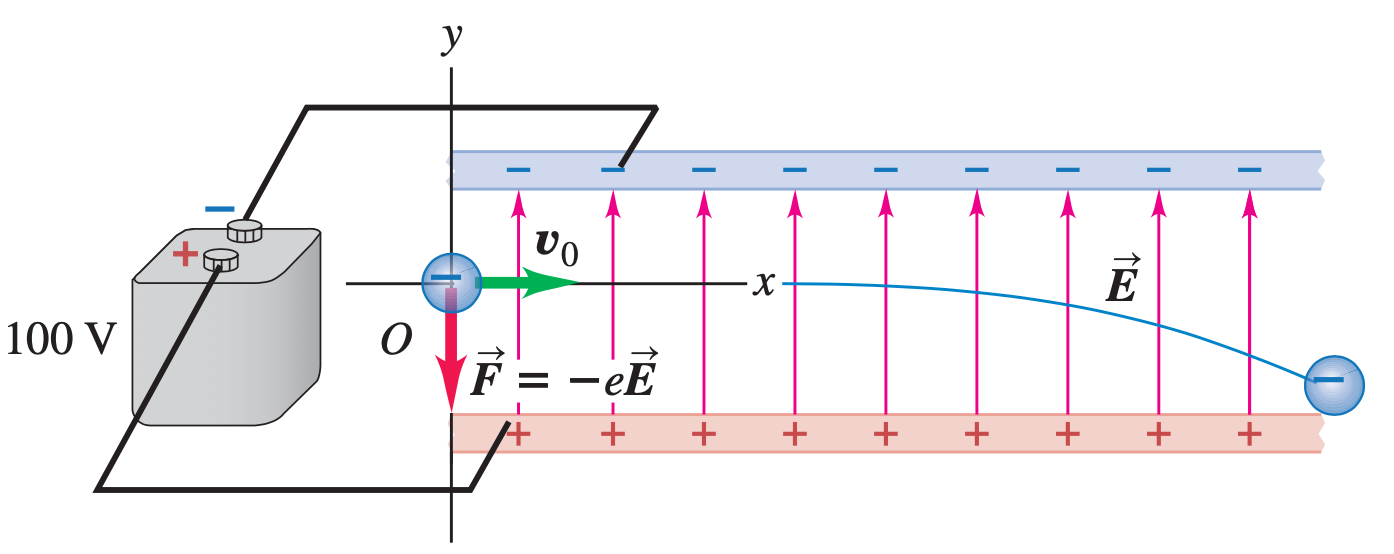
\includegraphics[width=.9\textwidth]{imagenes/imagenes22/T22IM20.png}
\end{figure}
\end{prob}

$a_x=0;\ MRU$ en eje $x$;  $\ a_y=-eE/m=cte;\ MRUA$ en eje $y$. $x_0=y_0=0;\ v_{0_x}=v_0; v_{0_y}=0$

$x=v_0t;\ quad y=\dfrac 1 2 a t^2=\dfrac 1 2 \dfrac{-eE}{m} t^2$

Eliminando $t$ de ambas ecuaciones: $\quad y=-\dfrac 1 2 \dfrac{eE}{mv_0^2}\ x^2$, que es la ecuación de una parábola hacia abajo, similar a la del tiro horizontal vista en el capítulo 2. La curvatura depende de la intensidad del campo $E$.

Si se invierten los signos de las cargas en las placas, se invierte la dirección del campo y la trayectoria del electrón sería una curva parabólica hacia arriba. Se puede dirigir el electrón variando la carga en las placas y esto se utiliza para controlar la trayectoria de los haces de electrones en los osciloscopios.

\begin{prob}
Se lanza un electrón con velocidad $v_0=2\times 10^7	 \ \mathrm{m\ s}^{-1}$ en la dirección de un eje equidistante de las placas planoparaleleas de un tubo de rayos catódicos, como se ve en la figura.

\begin{figure}[H]
	\centering
	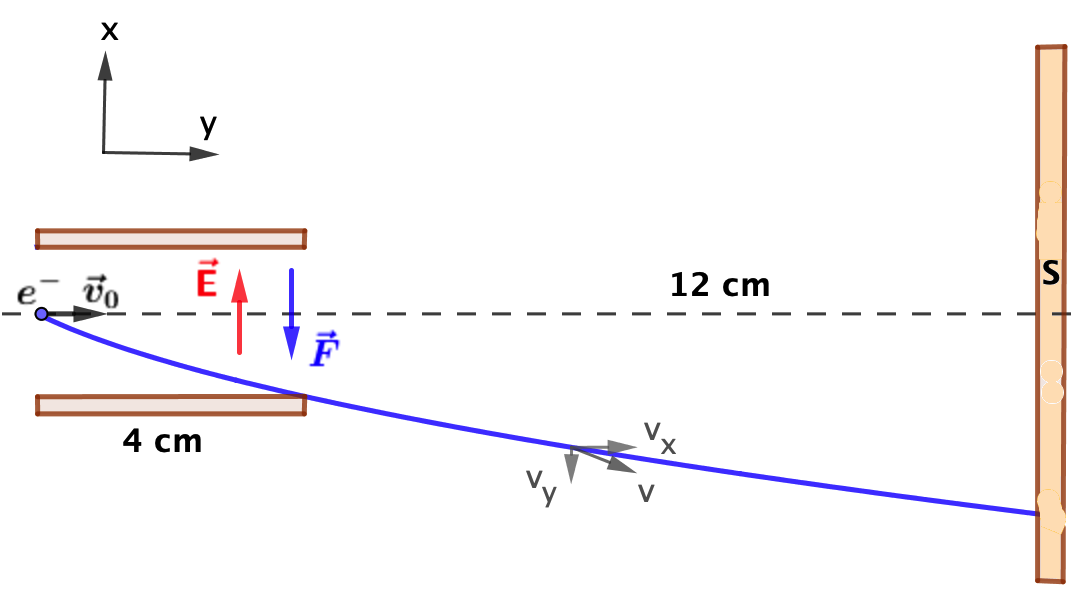
\includegraphics[width=.8\textwidth]{imagenes/imagenes22/T22IM17.png}
\end{figure}

El campo eléctrico uniforme entre las placas tiene una intensidad de $E = 2\times 10^{4} \ \mathrm{N \ C}^{-1}$ y está dirigido hacia arriba.

 ?`Qué distancia perpendicular al eje ha recorrido el electrón cuando pasa por el extremos de las placas?
 ?`Cuál es el ángulo con el eje que forma su velocidad cuando abandona la placa?
?`A qué distancia, por debajo del eje, choca contra la pantalla fluorescente S?

\end{prob}

$E=cte \to MRUA$ en eje $Y$, en eje $x \ MRU$

Tiempo en recorrer las placas, $t_p: \quad t_p=\dfrac x {v_x}=\dfrac{4\times 10^{-2}}{2\times 10^7}=2\times 10^{-9} \ \mathrm{s}$

Movto. eje $y:\quad F=eE=cte=ma \to a=\dfrac{2y}{t^2} \to m_e\dfrac{2y}{t^2}=eE \to$

$ y=\dfrac{eEt^2}{2m_e}=0,7035\times 10^{-2} \ \mathrm{m}$

$v_y=\cancelto[0]{v_{0_y}}+at \to v_y=\dfrac{2y}{t^2}t=\dfrac{2y}{t}=0.7035\rtimes 10^{7}\ \mathrm{m\ s}^{-1}$

Eje $x$, MRU: $\ v_x=v_{0_x}=2\times 10^7\ \mathrm{m\  s}^{-1} \ \to \ \tan \alpha=\dfrac{v_y}{v_x}=0.351 \ \to \ $

$\alpha=19.05ô$

Tiempo en llegar a la pantalla 

$S: \quad t_S=\dfrac{x}{v_x}=\dfrac{12\times 10^{-2}}{2\times 10^{-7}}=6\times 10^{-9} \ \mathrm{m\ s}^{-1}$ 

Al abandonar la placa el electrón no está sometido a fuerza alguna: 

$F=0\to a=0 \to MRU: \quad $

$y=\cancelto{0}{y_0}+v_y t=0.6035\times 10^2 \cdot 6 \times 10^{-9}=4.9245\times 10^{-2} \ \mathrm{m}=4.9225 \ \mathrm{cm}$.

\begin{prob}
Dos bolas iguales en masa $m$ están cargadas con una carga $q$ y cuelgan de sendos hilos de seda de longitud $L$ de un mismo punto. Determinar la distancia $x$ que separa a las bolas cuando el ángulo de separación es muy pequeño.	
\end{prob}

\begin{multicols}{2}
$\tan \theta=\dfrac{x/2}{L\cos \theta}=\dfrac{F_e}{mg}$

$\dfrac{x/2}{L\cos \theta}=\dfrac{q/(4\pi \varepsilon_0 x^2)}{mg}$

$x^3=\dfrac{q^2L\cos \theta}{2\pi \varepsilon_0 m g}$

$\theta << 1 \to \cos \theta \approx 1$

$x\approx \sqrt[3]{\dfrac{q^2L}{2\pi \varepsilon_0 m g}}$
\begin{figure}[H]
	\centering
	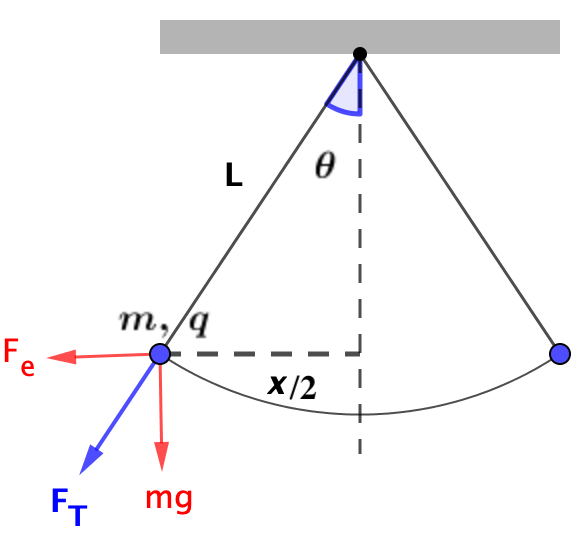
\includegraphics[width=.5\textwidth]{imagenes/imagenes22/T22IM18.png}
\end{figure}	
\end{multicols}


\begin{prob}
El electroscopio es un instrumento que se usa para saber si un cuerpo está cargado eléctricamente.

Un modelo simplificado de electroscopio consiste en dos pequeñas esferas de madera de masa $m$ con cargas iguales $q$ que cuelgan de dos hilos de longitud $l$. A partir de la mediada del ángulo de separación $2 \theta$ de las las esferas se puede calcular la carga $q$.
\end{prob}
\begin{multicols}{2}
Sobre cada peso actúan tres fuerzas: $\ F_p=mg,$ peso; $\ F_e=F, $ fuerza eléctrica; ; $\ T$, tensión del hilo.

$T \sin\theta = F;\ \  T\cos \theta =mg$

Dividiendo: $\ \tan \theta = \dfrac F{mg} \to $

$F=mg\tan \theta$

$r/2=l\sin \theta \to r=2l\sin \theta$
$F=\dfrac{q^2}{4\pi \varepsilon_0 r^2}=\dfrac{q^2}{4\pi \varepsilon_0 (2l\sin \theta)^2}$
\begin{figure}[H]
	\centering
	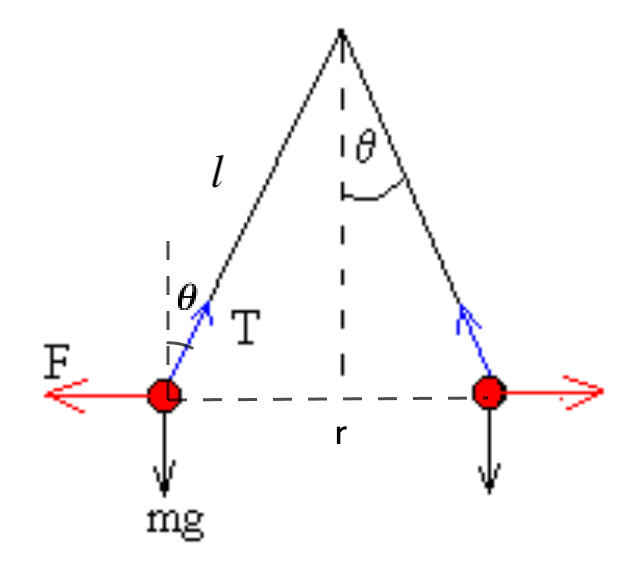
\includegraphics[width=.5\textwidth]{imagenes/imagenes22/T22IM25.png}
\end{figure}	
\end{multicols}

$q=\sqrt{F4\pi \varepsilon_0 (2l\sin \theta)^2}=4l\sin \theta \sqrt{\pi \varepsilon_0 m g \tan \theta}$



\begin{prob}
Un conductor en forma de anillo con radio $a$ tiene una carga total $Q$ distribuida de manera uniforme en todo su perímetro. Encuentre el campo eléctrico en el punto $P$ que se localiza sobre el eje del anillo a una distancia $x$ del centro.	
\begin{figure}[H]
	\centering
	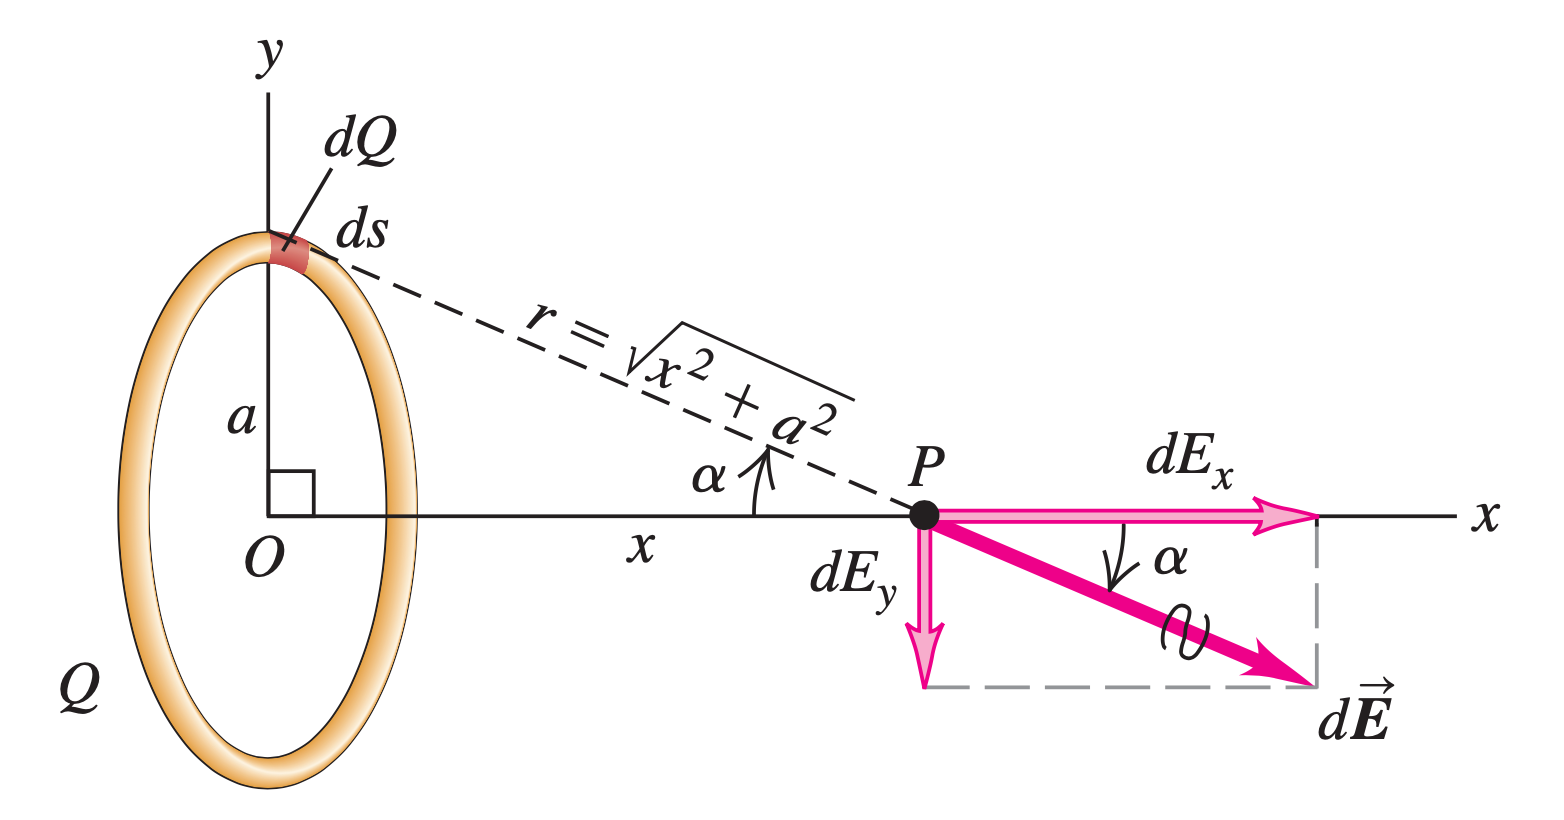
\includegraphics[width=.9\textwidth]{imagenes/imagenes22/T22IM21.png}
\end{figure}
\end{prob}
El cálculo de $\vec E$ en el eje de simetría del anillo se simplifica mucho. Las contribuciones al campo $\dd \vec E$ de los elementos de longitud $\dd s$, en el eje $y$ se anulan y solo quedan contribuciones en el eje $x$, así que $\vec E$ solo tendrá componente en el eje $x$, $E_y=E_z=0$

De la figura: $\ r^2=x^2+a^2 \ \to \ \dd E=\dfrac{1}{4\pi \varepsilon_0} \dfrac{\dd Q}{x^2+a^2}$

La componente $x$ de este campo eléctrico elemental será:

$\dd E_x=\dd E \cos \alpha = \dfrac{1}{4\pi \varepsilon_0} \dfrac{\dd Q}{x^2+a^2} \dfrac x r =\dfrac{1}{4\pi \varepsilon_0} \dfrac{\dd Q}{x^2+a^2} \dfrac {x} {\sqrt{x^2+a^2}} $

$\dd E_x=\dfrac{1}{4\pi \varepsilon_0} \dfrac{x\ \dd Q}{(x^2+a^2)^{(3/2)}}$

Integrando a lo largo de todo el anillo: $\ E_x=\displaystyle \int_Q \dfrac{1}{4\pi \varepsilon_0} \dfrac{x\ \dd Q}{(x^2+a^2)^{(3/2)}}$  

Como $x$ no varía a medida que recorremos el anillo, puede salir fuera y la integral queda como:

$\vec E = E_x \vec i=\displaystyle  \dfrac{1}{4\pi \varepsilon_0} \dfrac{x}{(x^2+a^2)^{(3/2)}} \ \int_Q \dd Q  \ \vec i = 
 \dfrac{1}{4\pi \varepsilon_0} \dfrac{x\ Q}{(x^2+a^2)^{(3/2)}} \vec i$ 
 
 \textbf{Análisis de casos extremos:}
 
 --- En el centro del anillo, $x=0$, el campo es cero, como era de esperar. Las contribuciones al campo de los elemento de longitud diametralmente opuestos se anulan y el campo total es cero.
 
 --- Cuando estamos sobre el eje de simetría muy lejos del anillo, $x>>a$, el denominador tiende a $x^3$ y el campo vale: 
 $E= \frac{1}{4\pi \varepsilon_0} \frac Q {x^2}\vec i$,
 como el campo que generaría una carga puntual $Q$ situada en el centro del anillo, el anillo parecería como un punto cargado.

\begin{prob}
Calcula el campo eléctrico que genera un disco de radio $R$	con densidad superficial de carga positiva y uniforme $\sigma$, en un punto a lo largo del eje del disco que esté a una distancia $x$ de su centro.
\begin{figure}[H]
	\centering
	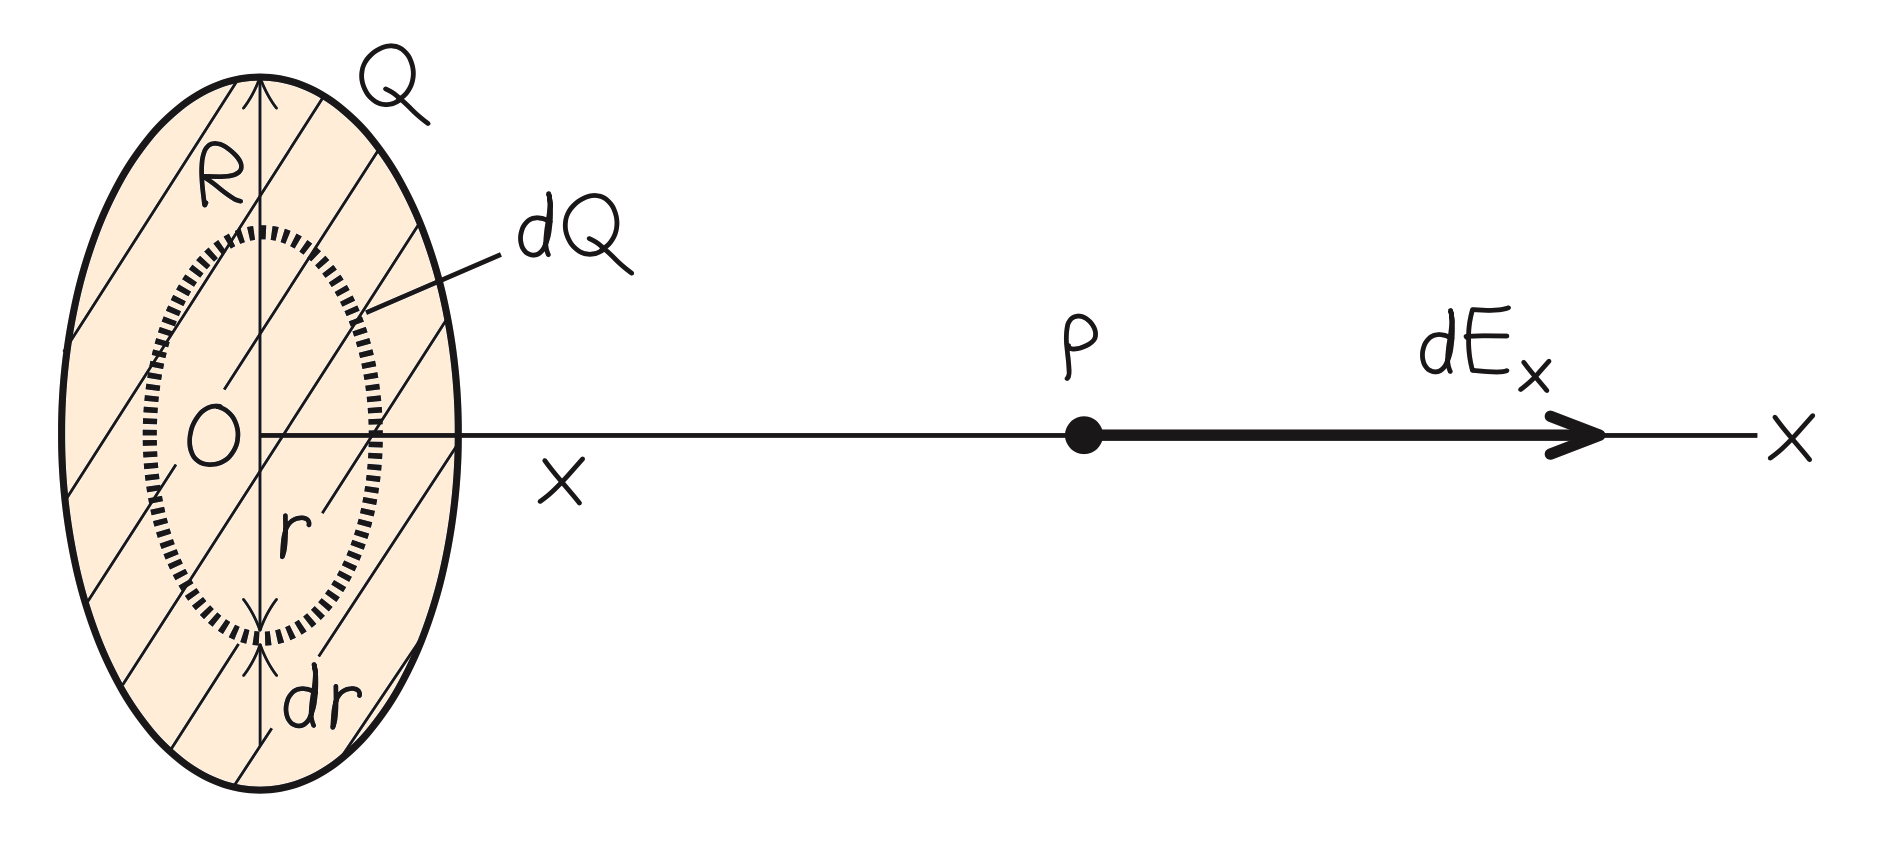
\includegraphics[width=.9\textwidth]{imagenes/imagenes22/T22IM22.png}
\end{figure}
\end{prob}

Como en el caso anterior y debido a la simetría de la distribución de carga, solo habrá contribución al campo en el eje $x,\ \vec E=E_x\ \vec i$.

Consideramos el anillo formado por anillos infinitesimales concéntricos de radio $r$ y espesor $\dd r$ y con una carga $\dd q$.

$\dd A= 2\pi r \dd r; \qquad \sigma=\dfrac Q{4\pi R^2}=\dfrac{\dd q}{\dd A} \ \to \ \dd q= \sigma \dd A=\sigma 2 \pi r \dd r$. 

Con $r$ variando desde $0$ hasta $R$

El campo que en el eje $x$ crea uno de estos anillos elementales es,  cambiando el radio del anillo anterior $a$ por $r$ y $Q$ por $\dd q$:

$\dd Ex=\dfrac{1}{4\pi \varepsilon_0} \dfrac{x\ \dd q}{(x^2+r^2)^{3/2}}=
\dfrac{1}{4\pi \varepsilon_0} \dfrac{x \ 2\pi \sigma r \dd r}{(x^2+r^2)^{3/2}}$

Como $x$ no varia al cambiar el $r$ del anillo, integrando desde que $r=0$ hasta $r=R$ para contar las contribuciones de todos los anillos elementales:

$\displaystyle E_x= \dfrac{\sigma x}{2\varepsilon_0}\int_0^R \dfrac{r\ \dd r}{(x^2+r^2)^{3/2}}=\dfrac{\sigma x}{2\varepsilon_0} \ \dfrac 1 2 \ \left[ \eval{ \dfrac{(x^2+r^2)^{(-1/2)}}{-1/2} }_0^R \right.$

$E_x=\displaystyle
\dfrac{\sigma x}{2 \varepsilon_0} \left| \eval{-\dfrac 1 {\sqrt{x^2+R^2}}}_0^R \right.= \dfrac {\sigma x}{2\varepsilon_0} \left[ -\dfrac{1}{\sqrt{x^2+R^2}}+\dfrac 1 x \right]$

$\vec E=E_x\ \vec i = \dfrac{\sigma}{2\varepsilon_0} \left[ \dfrac x x - \dfrac x{\sqrt{x^2+R^2}}\right]= \dfrac{\sigma}{2\varepsilon_0} \left[ 1-\dfrac 1{\sqrt{1+ \dfrac {R^2}{x^2}}} \right]$


Si aumenta indefinidamente el radio del disco $R$ aumentando proporcionalmente la carga para que se la densidad de carga se mantenga constante, $R>>x$ y el término que resta en el corchete es despreciable frente a la unidad, por lo que $\vec E=\dfrac{\sigma}{2	\varepsilon_0}\ \vec i=cte \vec i$, no depende de a distancia $x$ y queda como el campo eléctrico creado por una lámina cargada plana e infinita siendo la dirección del campo perpendicular a la placa en cualquier punto. \textcolor{gris}{Esto se verá en el próximo tema con el teorema de Gauss y la definición del flujo eléctrico.}

\begin{prob}
Se colocan dos láminas infinitas y planas paralelas entre sí, separadas por una distancia $d$ (ver figura). La lámina inferior tiene una densidad superficial de carga uniforme y positiva $\sigma$, y la lámina superior tiene una densidad superficial de carga uniforme y negativa $-\sigma$, ambas de la misma magnitud. Encuentre el campo eléctrico entre las dos láminas, arriba de la lámina superior y debajo de la lámina inferior.	
\end{prob}
\begin{figure}[H]
	\centering
	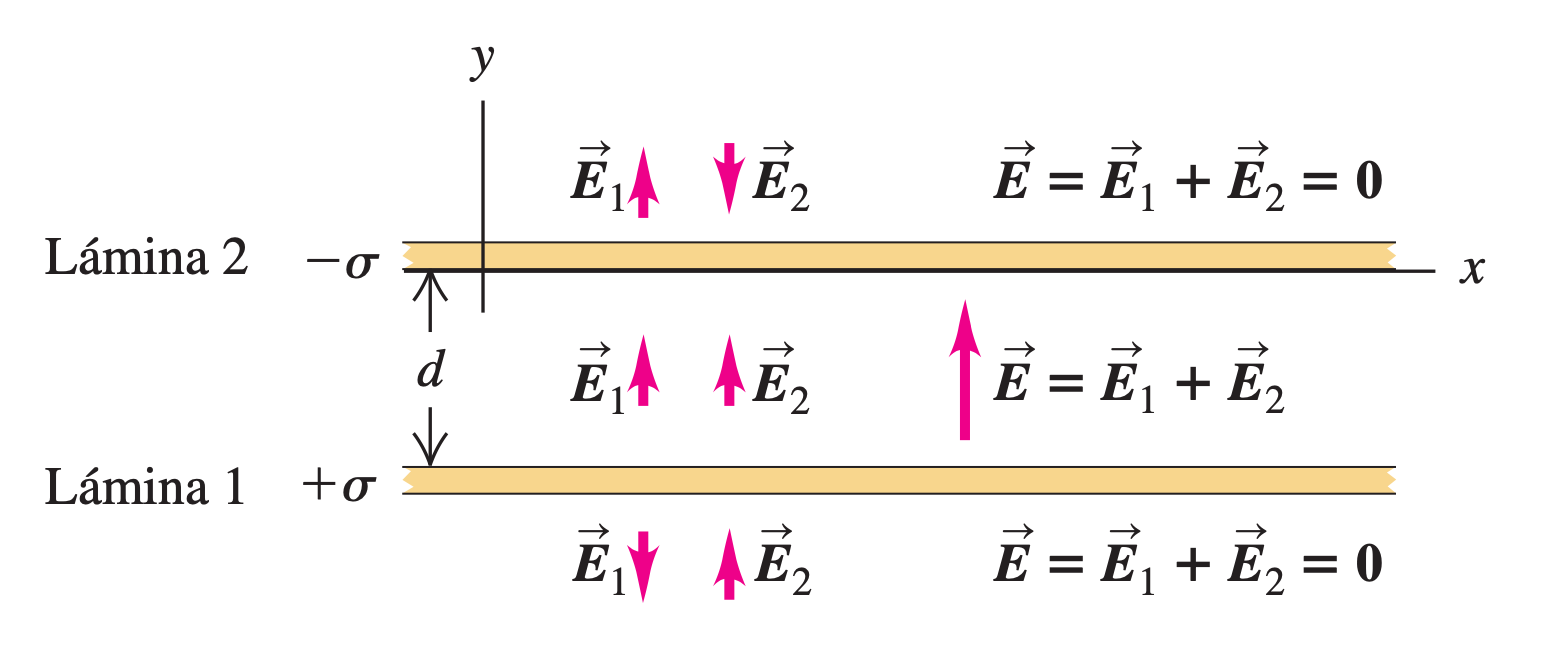
\includegraphics[width=1\textwidth]{imagenes/imagenes22/T22IM24.png}
\end{figure}

Del problema anterior sabemos cuál es el campo creado por una sola lámina cargada, plana e infinita. Ahora debemos encontrar cuál es el campo que crean dos de estas láminas y para ello usaremos el principio de superposición.

Sin importar la distancia a la lámina, tenemos que $E_1=E_2=\dfrac{\sigma}{2\varepsilon_0}$. $\vec E_1$ se aleja de la carga positiva y $\vec E_2$ se acerca a la caga negativa, ambos en la dirección $\vec j$. Entre las láminas, los campos se refuerza; fuera de ellas, se cancelan mutuamente, como se ve en la figura.

$$\vec E=\vec E_1+\vec E_2=\begin{cases}
\ 0 & \text{arriba lámina superior}	 \\
\ \dfrac{\sigma}{2\varepsilon_0} \vec j & \text{entre las láminas} \\
\ 0 & \text{abajo lámina inferior}
\end{cases}$$


\begin{prob}
Una carga eléctrica, $Q$, positiva está distribuida uniformemente a lo largo de una línea con longitud de $2a$ que se ubica sobre el eje $y$, entre $y=-a$ y $y=+a$ (ver figura). Calcule el campo eléctrico en el punto $P$ sobre el eje $x$, a una distancia $x$ del origen
\end{prob}
El eje $x$ es la mediatriz del segmento de carga.
\begin{multicols}{2}
	Como en problemas anteriores, por la simetría del problema, solo habrá campo en la componente $x$. En el ejes $y$, las contribuciones al campo de elementos del segmento en la posición $y$ se cancelan con las situadas en la posición $-y$, por lo que $E_y=0$, por razonamientos análogos de simetría, $E_z=0$. Conclusión: $\vec E = E_x \ \vec i$
\begin{figure}[H]
	\centering
	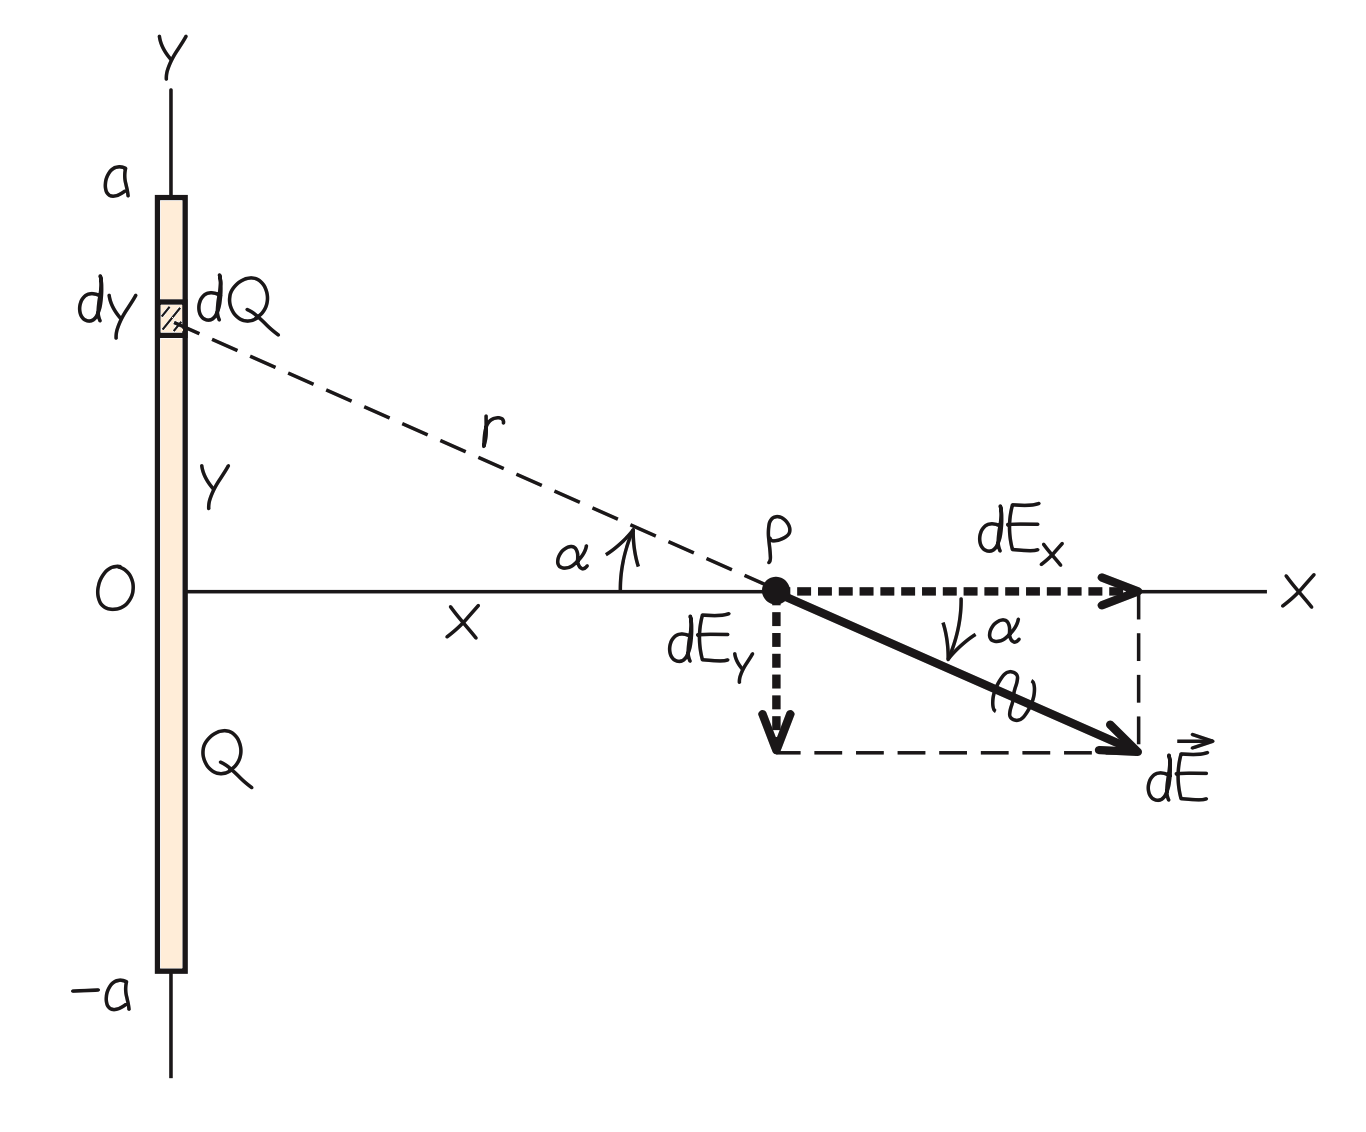
\includegraphics[width=.55\textwidth]{imagenes/imagenes22/T22IM23.png}
\end{figure}
\end{multicols}
$\lambda:$ densidad lineal de carga.  $\quad \lambda=\dfrac Q{2a}=\dfrac{\dd q}{\dd y} \ \to \dd q=\lambda \ \dd y=\dfrac{Q}{2a} \ \dd y$
 
La distancia $r$ entre el elemento de línea de carga y el punto $P$ donde queremos calcular el campo es: $\ r=\sqrt{x^2+y^2}$, por lo que la contribución al campo de este elemento de línea será:

$\dd E=\dfrac 1 {4\pi \varepsilon_0} \dfrac{\dd Q}{r^2}=\dfrac Q {4\pi \varepsilon_0} \dfrac{\dd y}{2a(x^2+y^2)}$

Como $\cos \alpha=\dfrac{x}{r}=\dfrac{x}{\sqrt{x^2+y^2}} \to \dd E_x=\dd E \cos \alpha$

$\dd E_x=\dfrac Q {4\pi \varepsilon_0} \dfrac{x\dd y}{2a(x^2+y^2)^{3/2}}$

Para calcular el campo total, integramos desde $y=-a$ hasta $y=+a$.

$\displaystyle E=\dfrac 1 {4\pi \varepsilon_0} \dfrac{Qx}{2a} \int_{-a}^{+a} \dfrac{\dd y}{(x^2+y^2)^{3/2}}$, integral que requiere el cambio trigonométrico $y/x=sin t$ o se puede consultar en una tabla.

$\vec E=E_x \ \vec i = \dfrac Q {4\pi \varepsilon_0} \ \dfrac{1}{x \ \sqrt{x^2+a^2}} \ \vec i$


\textbf{análisis de casos extremos:}

--- $x>>a\ \to \ \vec E= \dfrac 1 {4\pi \varepsilon_0} \dfrac{Q}{x^2} \vec i$. 

Si $P$ está muy lejos del segmento cargado, éste se comporta como una carga puntual situada en el punto medio del segmento.

---$x<<a$, escribimos $\vec E $ en función de la densidad lineal de carga $\lambda=Q/2a$,

$\vec E=E_x \ \vec i = \dfrac 1 {2\pi \varepsilon_0} \ \dfrac{\lambda}{x \ \sqrt{(x^2/a^2)+1}} \ \vec i \approx \dfrac{\lambda}{2\pi \varepsilon_0}\ \vec i$

El campo solo depende de la distancia al punto $P$ de la línea de carga, luego, a una distancia $r$ de la línea \emph{infinita} de carga, el campo será:

$E=\dfrac{\lambda}{2\pi \varepsilon_0 r}$

El campo de una línea infinita de carga varia como $1/r$, no como $1/r^2$ como lo hace una carga puntual. Para $\lambda>0$ el campo es hacia afuera de la línea y hacia adentro para $\lambda <0$.

Esta aproximación es válida cuando $r<<a$, por ejemplo, si la distancia $r$ de donde calculamos el campo a la línea que lo origina es del $1\%$ de la longitud de ésta, el valor de la aproximación de $E$ difiere del valor del campo que crearía un segmento finito en menos del $0.02\ \%$.

\begin{prob}
Hallar el potencial y el campo eléctrico en un pinto situado sobre el eje de un disco de radio R que tiene una densidad de carga $\sigma$ por unidad de superficie.	
\end{prob}

Debido a la simetría de la distribución de carga, solo habrá contribución al campo en el eje $x,\ \vec E=E_x\ \vec i$. (ver problema 22.9)

Consideramos el anillo formado por anillos infinitesimales concéntricos de radio $r$ y espesor $\dd r$ y con una carga $\dd q$.

\begin{figure}[H]
	\centering
	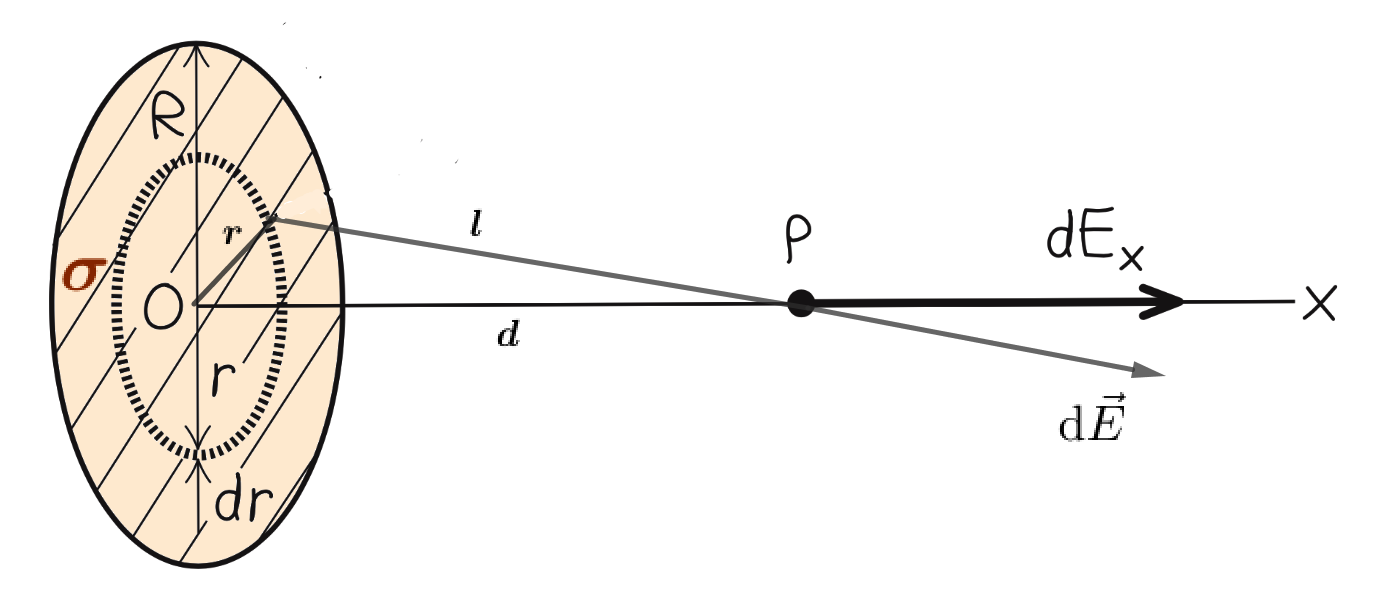
\includegraphics[width=.9\textwidth]{imagenes/imagenes22/T22IM26.png}
\end{figure}

$\dd q=\sigma 2 \pi r \dd r \ \to \ \dd V= \dfrac{\sigma 2 \pi r \dd r}{4\pi \varepsilon_0 \sqrt{r^2+d^2}}$

$\displaystyle V=\int_0^R \dfrac{\sigma  \pi r \dd r}{\pi \varepsilon_0 \sqrt{r^2+d^2}}=\dfrac {\sigma}{\boldsymbol{ 2}\varepsilon_0} \int_0^R \dfrac{\sigma \boldsymbol{ 2} \pi r \dd r}{2\pi \varepsilon_0 \sqrt{r^2+d^2}}=\dfrac{sigma}{2\varepsilon_0} \left[ \sqrt{r^2+d^2} \right]_0^R=\dfrac{\sigma}{2\varepsilon_0} \sqrt{\sqrt{R^2+d^2}-d}$

$E_-\displaystyle \dv{V}{x}=-\dfrac{\sigma}{2\varepsilon_0} \left[ \dfrac {d}{\sqrt{R^2+d^2}} -1 \right]$

\newpage %********************************************

\begin{myblock}
{\small{Formas para cambiar la carga eléctrica de los cuerpos}}

\small{Se denomina electrización al efecto de ganar o perder cargas eléctricas, normalmente electrones, producido por un cuerpo eléctricamente neutro. Los tipos de electrificación son los siguientes:}
\begin{itemize}
\item \small{Electrización por contacto: Cuando ponemos un cuerpo cargado en contacto con un conductor se puede dar una transferencia de carga de un cuerpo al otro y así el conductor queda cargado, positivamente si "cedió electrones" o negativamente si los "ganó".}
\item \small{Electrización por fricción: Cuando frotamos un aislante con cierto tipo de materiales, algunos electrones son transferidos del aislante al otro material o viceversa, de modo que cuando se separan ambos cuerpos quedan con cargas opuestas.}
\item \small{Carga por inducción: Si acercamos un cuerpo cargado negativamente a un conductor aislado, la fuerza de repulsión entre el cuerpo cargado y los electrones de valencia en la superficie del conductor hace que estos se desplacen a la parte más alejada del conductor al cuerpo cargado, quedando la región más cercana con una carga positiva, lo que se nota al haber una atracción entre el cuerpo cargado y esta parte del conductor. Sin embargo, la carga neta del conductor sigue siendo cero (neutro).}
\begin{figure}[H]
	\centering
	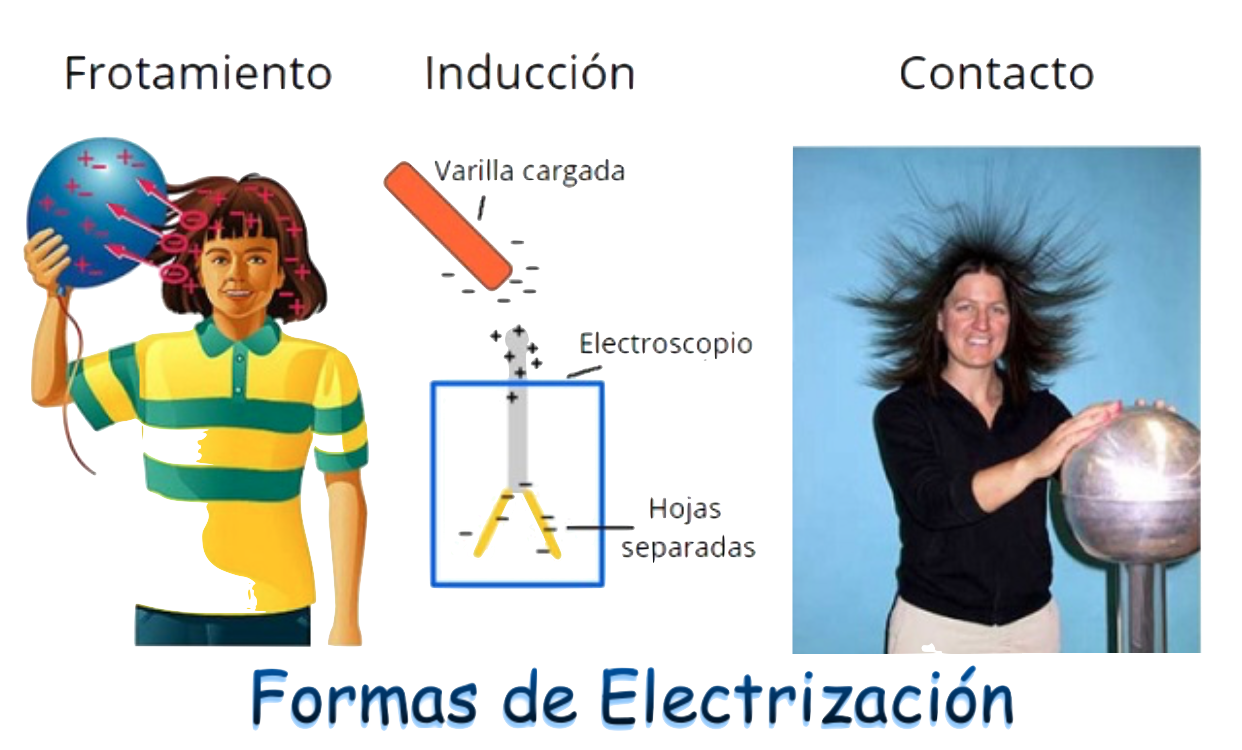
\includegraphics[width=.9\textwidth]{imagenes/imagenes22/T22IM12.png}
\end{figure}
\item \small{Carga por el efecto fotoeléctrico: Sucede cuando se liberan electrones en la superficie de un conductor al ser irradiado por luz u otra radiación electromagnética.}
\item \small{Carga por electrólisis: Descomposición química de una sustancia, producida por el paso de una corriente eléctrica continua.}
\item \small{Carga por efecto termoeléctrico: Significa producir electricidad por la acción del calor}\normalsize{.}
\end{itemize}	

\end{myblock}









